\documentclass[main.tex]{subfiles}

\begin{document}

\addtocontents{toc}{\let\protect\contentsline\protect\nopagecontentsline}
\chapter{Numerical}\label{cpt:num}
\addtocontents{toc}{\let\protect\contentsline\protect\oldcontentsline}

While the previous chapter introduced the formalism for parton branchings in vacuum and medium, we will now turn to a numerical treatment of the evolution equations. This will be done by using the results of the previous chapter to build a Monte-Carlo program for simulating parton showers, both for vacuum and medium cascades. Each section will be structured in the same manner, starting by determining how the cascade evolves relative to the branching probability, then developing methods for sampling random energy fractions from the splitting functions, and finally implementing this into Monte-Carlo programs. The results obtained from these programs will then be compared with the analytical results derived in \autoref{cpt:ana}, and used to highlight different properties of the cascades.

\section{Monte-Carlo for Parton Branching in Vacuum}
Starting by creating the Monte-Carlo programs for the vacuum cascades, where we want to develop one for pure gluon cascades (only \(gg\) splittings), and one for both quarks and gluons. The former will be created using the simplified \(gg\) splitting function, which can then be compared to the analytical results of the DGLAP cascade. The latter will be done using the full splitting functions, sampled using the \emph{Metropolis-Hastings algorithm} (MH), and will give us a more realistic picture of the branching process but no exact analytical solution to compare with.

\subsection{Evolution interval }\label{sec: determining_evolution_time_from_sudakov}
For our Monte-Carlo programs we need to determine the limits of the evolution variable \(t\), such that we know when to terminate a given shower. Recalling the evolution variable defined in \autoref{eqn: evolution_variable_vacuum}, and that our jets evolve in angle from some initial jet radius \(R\), down to the minimum angle \(\theta_{\text{min}} = Q_0/p_t\), with boundary values of the evolution variable given by \autoref{eqn: evolution_variable__limits_vacuum}. A plot of the maximum value for \(t\) for a given range of \(p_t\) and \(R\) values is given by \autoref{fig: evolution_variable_vacuumshowers}. Here it is apparent that most values of \(t\) are below \(0.4\).
\begin{figure}[htb]
    \centering
    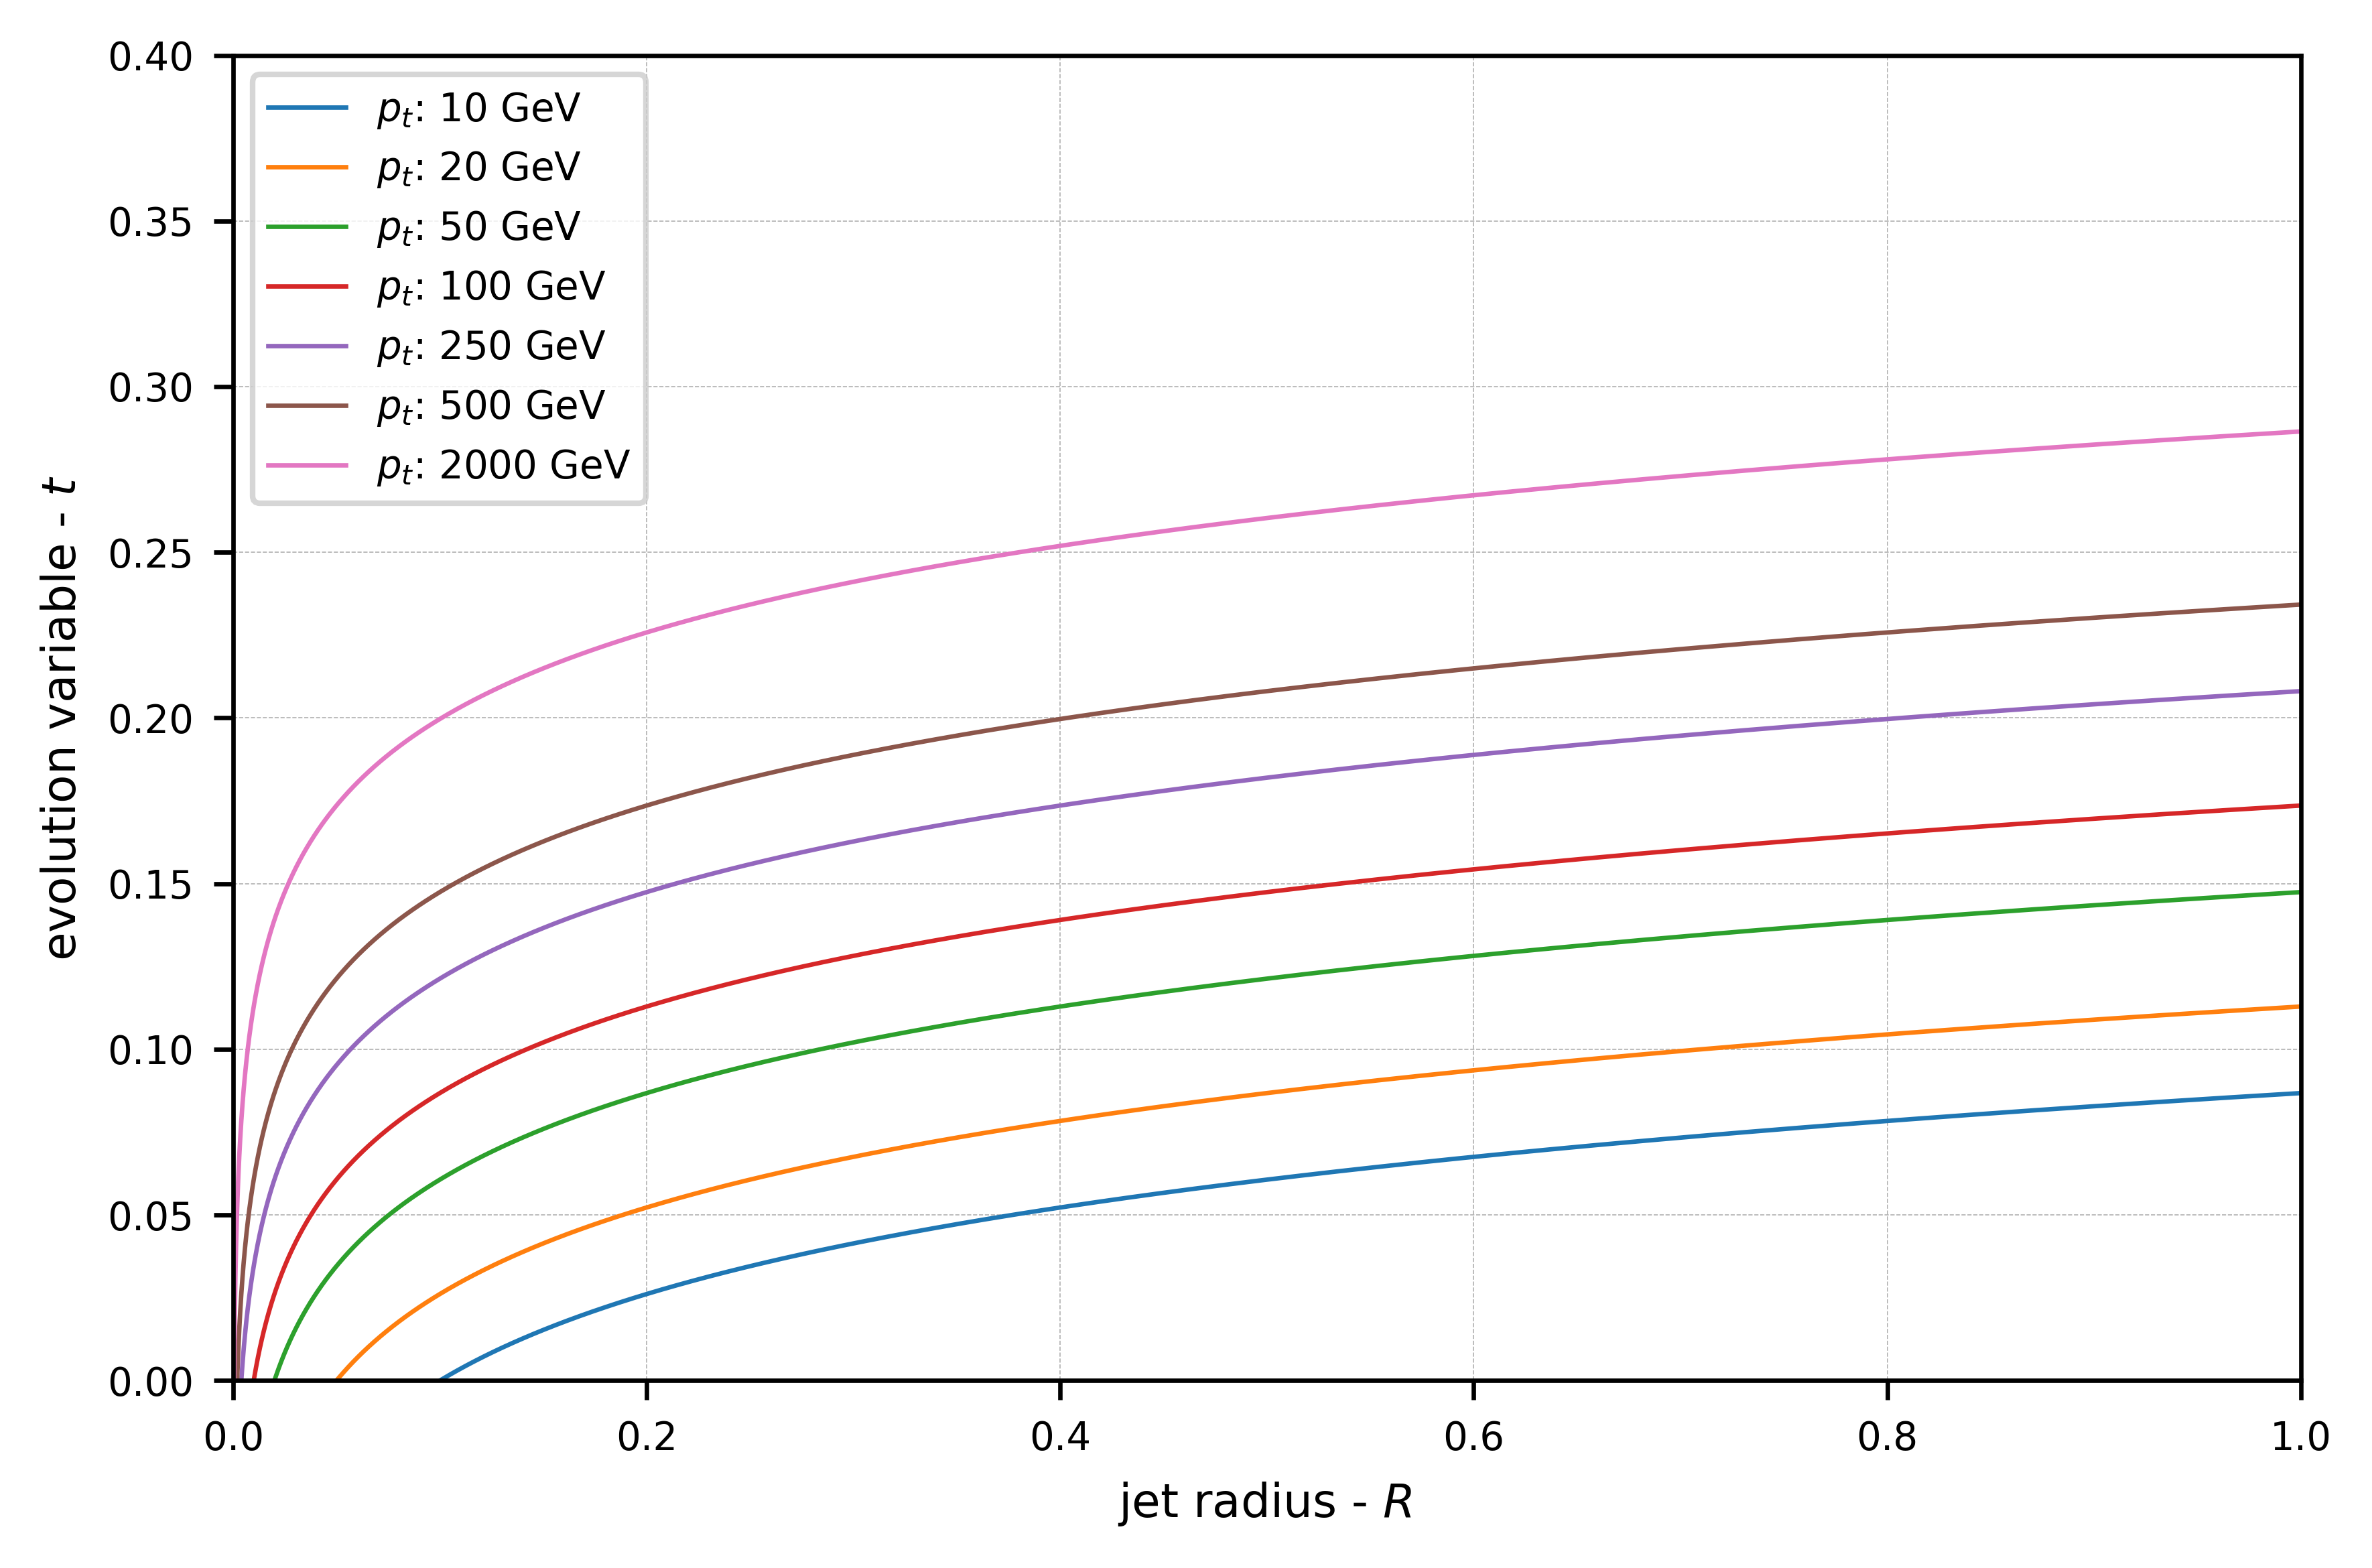
\includegraphics[width=9cm]{pictures/plots/misc/evolution_variable_vacuumshowers.png}
    \caption{Maximum values of the evolution variable \(t\) for vacuum showers, plotted up to \(p_t\,R > Q_0\). The strong coupling is set constant \(\alpha_s = 0.1184\) and \(Q_0 = 1 GeV\). Not that most values of \(t\) are well below \(0.4\). }
    \label{fig: evolution_variable_vacuumshowers}
\end{figure}

Knowing the boundaries we need to impose on the evolution variable for our Monte-Carlo, we can now move on to determining how to sample intervals of the evolution variable from the Sudakov form factor. As discussed in \autoref{cpt:ana}, the Sudakov form factor gives us the probability of no branching to occur in a given interval, so it is the natural candidate for generating random values of \(\Delta t\). Writing the Sudakov from \autoref{eqn: sudakov_form_factor_dasguptalike} in terms of the probability of splitting in the interval \(\mathcal{P}(\Delta t)\), in a given interval \(\Delta t\) 
\begin{equation}\label{eqn: branching_probability_from_sudakov_gg}
    \mathcal{P}(\Delta t) = \frac{\Delta(t)}{\Delta(t_0)} = \exp\left(-\Delta t \int_\epsilon^{1-\epsilon}dz \, P_{gg}(z)\right) 
\end{equation}
then it is trivial to rewrite the equation in terms of \(\Delta t\), and generate a random number in the interval \(\mathcal{P}(\Delta t) = \mathcal{R} \in [0,1]\), to obtain a random interval in which we can expect a new splitting
\begin{equation}\label{eqn: expected_branching_interval}
    \Delta t = -\frac{\ln(\mathcal{R})}{ \int_\epsilon^{1-\epsilon}dz \, P_{gg}(z)}.
\end{equation}
The expected splitting interval must be calculated for all the available partons. The parton which generates the smallest interval \(\Delta t\) is then expected to split first and will be the parton selected for splitting in our Monte-Carlo. 

\autoref{alg: evolution_boundaries} represents how our Monte-Carlo samples random evolution intervals, select a splitting parton, and imposes the boundary conditions of the evolution variable to determine when the terminate the shower. The general method outlined here is valid for all the vacuum programs, but \autoref{eqn: expected_branching_interval} is only valid for \(gg\)-branchings.
\begin{center}
\begin{minipage}{.8\linewidth}
\begin{algorithm}[H]
\caption{Evolution boundaries}
\label{alg: evolution_boundaries}
\begin{algorithmic}[1]
    \State calculate \(t_{\text{max}}\),
         \[t_{\text{max}} = \frac{\alpha_s}{\pi} \ln \frac{Rp_t}{Q_0}\]
    \While{\(t< t_{\text{max}}\)}
        \For{parton \textbf{in} AllPartons}
        \State calculate expected splitting interval. \[\Delta t = -\frac{ln(\mathcal{R})}{ \int_\epsilon^{1-\epsilon}dz \, P_{gg}(z)}\]
        \EndFor
    \State select the parton with shortest interval, \(\Delta t_{\text{min}} = \text{min}(\Delta t)\)
    \State evolve the angle \(t = t + \Delta t_{\text{min}}\).
    \EndWhile
\end{algorithmic}
\end{algorithm}
\end{minipage}
\end{center}

\subsection{Managing quarks and gluons}\label{sec: managing_quarks_and_gluons}
When creating a program with both quarks and gluons, the interval \(\Delta t\) must be advanced based on the type of parton being split. When splitting a gluon the interval will evolve according to the Sudakov given in \autoref{eqn: sudakov_vacuum_gluons}, and when splitting quarks the Sudakov is \autoref{eqn: sudakov_vacuum_quarks}. The branching probabilities are then calculated from the following equations
\begin{align}
    \mathcal{P}_{g}(\Delta t) &= \exp\left(-\Delta t \int_\epsilon^{1-\epsilon} \left[ P_{qg}(z) + P_{gg}(z) \right] \, dz \right)  \label{eqn: sudakov_splitting_interval_gluons}  \\
    \mathcal{P}_{q}(\Delta t) &= \exp\left(-\Delta t \int_\epsilon^{1-\epsilon} P_{qq}(z) \, dz \right). \label{eqn: sudakov_splitting_interval_quarks}
\end{align}
The question that remains is how to determine the splitting vertex when this parton is a gluon, as it can split with two different vertices. This can be done by comparing the contribution of the two vertices have on the available phase space
\begin{equation}\label{eqn: gluon_splitting_selection_ratios}
    W_{gg} = \frac{\int_\epsilon^{1-\epsilon} P_{gg}(z) \, dz}{\int_\epsilon^{1-\epsilon} \left[P_{qg}(z) + P_{gg}(z) \right]\, dz}.
\end{equation}
If the splitting parton is a gluon, we need to roll a random number \(\mathcal{R}\in[0,1)\), if the value \(\mathcal{R}< W_{gg}\), we will use the \(gg\) vertex, and if \(\mathcal{R}\geq W_{gg}\) it will be the \(qg\) vertex. When setting \(\epsilon = 10^{-3}\), the value is \(W_{gg} \approx 0.96\), so the vast majority of gluon splittings will be done via the \(gg\) vertex.

A similar comparison could have been done for the relative contributions on the total phase space for quarks and gluons, but this is already implemented into the calculations for \(\mathcal{P}_q(\Delta t)\), and \(\mathcal{P}_g(\Delta t)\), so this is not necessary. 

\subsection{Sampling from the vacuum splitting functions}\label{sec: metropolis_hastings}
The process of evolving the evolution variable, and selecting which parton and what vertex to use for each splitting, has now been outlined. The final piece of the Monte-Carlo puzzle is to determine how to sample random energy fractions from the splitting functions. This can be done if we consider the probability density of obtaining a parton with momentum fraction \(z\) as
\begin{equation}\label{eqn: probability_density_for_splitting}
    \mathcal{P}= \frac{ P_{ba}(z)}{\int_\epsilon^{1-\epsilon} dz \, P_{ba}(z)}.
\end{equation}
The probability \(\mathcal{P}\) can then be replaced with a randomly generated number, and the momentum fraction of the branched parton can be calculated from
\begin{equation}\label{eqn: energyfraction_function_R}
    \mathcal{R} \int_\epsilon^{1-\epsilon} dz \, P_{ba}(z) = \int_\epsilon^{y}dz \, P_{ba}(z).
\end{equation}
where \(\mathcal{R}\in [0,1]\)~\cite{ellis_stirling_webber_1996}. Note that since the splitting function is present on both sides of the equation, we can disregard any color and symmetry factors when calculating the splitting value, as they will not impact the final sample.

When trying to solve \autoref{eqn: energyfraction_function_R} for the different splitting functions, we will find that not all of them can be solved for a general momentum-fraction \(y\), and we need to introduce the Metropolis-Hastings algorithm for sampling them correctly~\cite{MCMC_andrieu2003}. The Metropolis-Hastings algorithm requires two different distributions,
\begin{enumerate}[1)]
    \item A target distribution \(P(x)\), which is the one we are trying to sample.
    \item A proposal distribution \(f(x)\) proportional to \(\mathcal{P}(x)\).
\end{enumerate}
The target distribution is naturally the full splitting function we are trying to sample. The proposal function will then be a \textit{dummy} splitting function, which is similar in shape to the full splitting function. Once these are chosen the Metropolis-Hastings algorithm is executed according to \autoref{alg: metropolis_hastings},
\begin{center}
\begin{minipage}{.8\linewidth}
\begin{algorithm}[H]
\caption{Metropolis-Hastings}
\label{alg: metropolis_hastings}
\begin{algorithmic}[1]
    \State sample a random value \(x'\) from \(f(x)\).
    \State calculate the acceptance probability, \[A(x') = \text{min} \left(1, \, \frac{P(x')}{f(x')}\right)\]
    \State generate a random number \(\mathcal{R}\in [0,1]\).
    \If{\(\mathcal{R}\leq A(x')\)} 
        \Statey accept the value \(x = x'\)
    \ElsIf{\(\mathcal{R} > A(x')\)} 
        \Statey reject the value \(x'\)
    \EndIf
\end{algorithmic}
\end{algorithm}
\end{minipage}
\end{center}

\subsubsection*{Sampling from the \(gg\) vertex}
When trying to solve \autoref{eqn: energyfraction_function_R} for the \(P_{gg}(z)\) splitting function in \autoref{eqn: vacuum_gg_splitting_function}, it is difficult to obtain an exact value of \(y\). It is therefore convenient to use the simplified splitting function of \autoref{eqn: vacuum_gg_simple_splitting_function} such that Metropolis-Hastings algorithm can be utilized. Excluding the color factor as it immediately cancels in the following calculation it can be written as
\begin{equation}\label{eqn: p_ggg_vacuum_dummy}
    P_{gg}^{\text{dummy}}(z) = \frac{1}{z(1-z)}
\end{equation}
and evaluating \autoref{eqn: energyfraction_function_R} to obtain a way of sampling values from this simplified splitting function. The integral is straightforward to execute
\begin{align}
    \mathcal{R} \int_\epsilon^{1-\epsilon} dz \, \frac{1}{z(1-z)} &= \int_\epsilon^{y} \frac{1}{z(1-z)}  \nonumber\\
    \mathcal{R} \left[ \ln (\frac{1-\epsilon}{\epsilon}) +   \ln(\frac{1-\epsilon}{\epsilon}) \right] &= \ln (\frac{y}{1-y}) +  \ln(\frac{1-\epsilon}{\epsilon}) \nonumber\\
    2\, \mathcal{R} \left[ \ln (\frac{1-\epsilon}{\epsilon}) \right] &= \ln (\frac{y}{1-y}  \frac{1-\epsilon}{\epsilon})
\end{align}
exponentiating both sides of the equation
\begin{align}\label{eqn: MC_energyfraction_origin_vacuum}
    \frac{y}{1-y} \frac{1-\epsilon}{\epsilon} &= \left(\frac{1-\epsilon}{\epsilon}\right)^{2\, \mathcal{R}} \nonumber\\
    \frac{y}{1-y} &= \left(\frac{1-\epsilon}{\epsilon}\right)^{2\, \mathcal{R}-1} \nonumber\\
    y &= \frac{\left(\frac{1-\epsilon}{\epsilon}\right)^{2\, \mathcal{R}-1}}{1+\left(\frac{1-\epsilon}{\epsilon}\right)^{2\, \mathcal{R}-1}}
\end{align}
and simplifying, gives an expression which can be used to randomly generate parton energy fractions from the simplified splitting function
\begin{equation}\label{eqn: MC_energyfraction_gg_vacuum}
    y(\mathcal{R}) = \frac{\xi}{1+ \xi} \qquad \text{for, } \quad \xi = \left(\frac{1-\epsilon}{\epsilon}\right)^{2\, \mathcal{R}-1}.
\end{equation}

Applying the Metropolis-Hastings algorithm by sampling the dummy splitting function according to \autoref{eqn: MC_energyfraction_gg_vacuum}, we can generate a plot of the original histogram, compared to the Metropolis-Hastings correction. This gives us a good idea of how the correction works and allows us to demonstrate how this simple algorithm allows us to sample more complex functions. The resulting plot is given in \autoref{fig: MH_corrected_p_gg_splitting}.
\begin{figure}[htb]
    \centering
    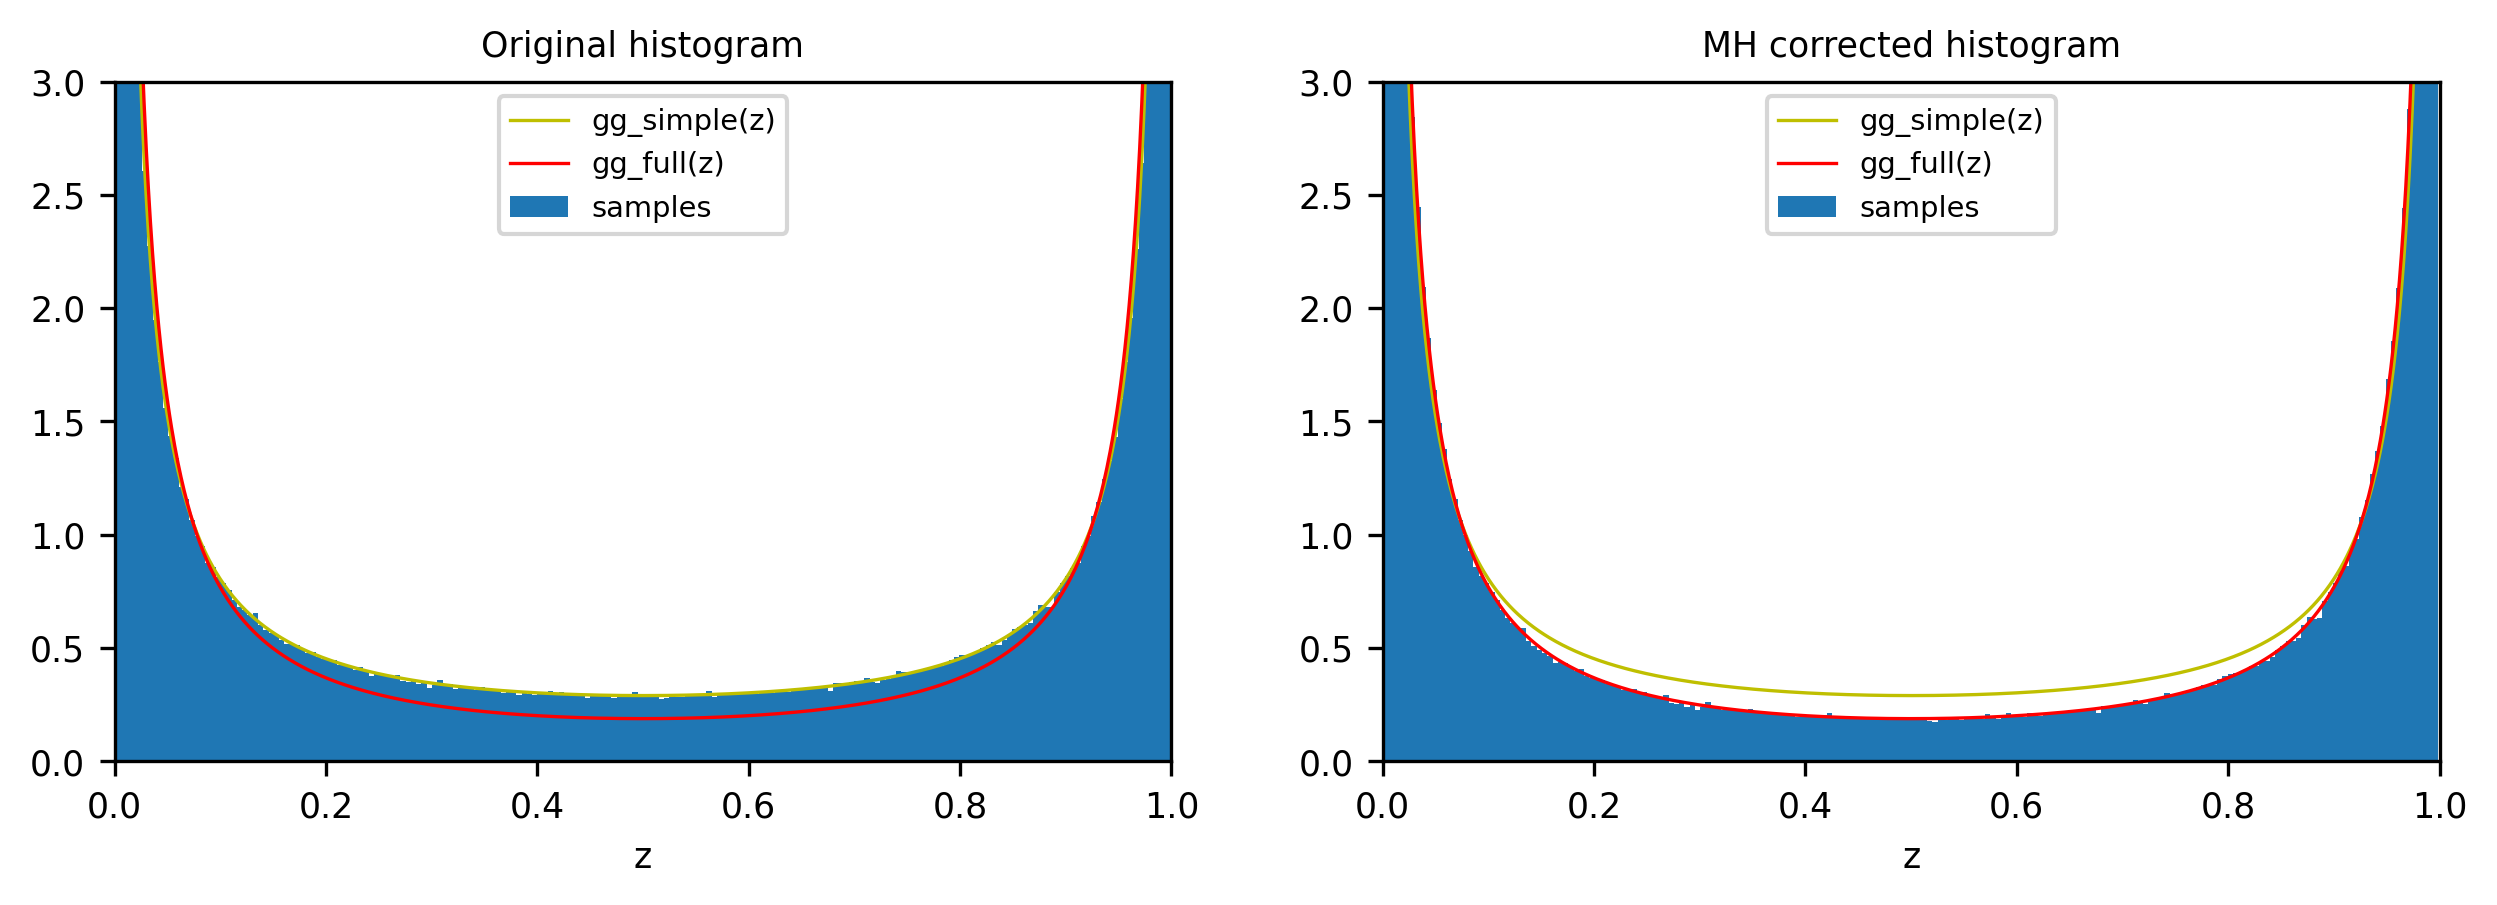
\includegraphics[width=15cm]{pictures/plots/Metropolis-Hastings/MH_vacuum_gg.png}
    \caption{Probability density of the full \(P_{gg}(z)\) splitting function and the dummy splitting function \(P_{gg}^{\text{dummy}}(z)\). The left plot gives the values sampled from \autoref{eqn: MC_energyfraction_gg_vacuum},and the right plot is corrected using Metropolis-Hastings algorithm. Simulated with \(10^6\) samples, and a MH acceptance rate of \(0.87\).}
    \label{fig: MH_corrected_p_gg_splitting}
\end{figure}

\subsubsection*{Sampling from the \(qg\) vertex}
Now we will find a way of sampling random values from the \(P_{qg}(z)\) splitting function given by \autoref{eqn: vacuum_qg_splitting_function}. In contrast to the other splitting functions, this one is actually not divergent such that \(\epsilon\) can be set equal zero. Solving \autoref{eqn: energyfraction_function_R} for \(P_{qg}(z)\),
\begin{align}
    \mathcal{R} \,\int_0^1 P_{qg}(z)dz &= \int_0^y P_{qg}(z)dz \nonumber \\
    \frac{2}{3}\,\mathcal{R} &= \left[ y - y^2 + \frac{2}{3} y^3 \right] \nonumber\\
    \frac{2}{3}\,\mathcal{R} &= y - y^2 + \frac{2}{3} y^3 \nonumber \\
    0 &= \frac{2}{3} y^3 - y^2 + y - \frac{2\, \mathcal{R}}{3} \label{eqn: gqq_vertex_qubic_formula}
\end{align}
This is a cubic formula. Setting \(d = \frac{2\, \mathcal{R}}{3} \), we can throw \autoref{eqn: gqq_vertex_qubic_formula} into WolframAlpha, and find the single real root to be,
\begin{equation}\label{eqn: gqq_vacuum_sample}
    y \approx 0.5 + 0.5 \left[(36 d^2 - 24 d + 5)^{1/2} + 6 d - 2\right]^{1/3} - \frac{0.5}{\left[(36 d^2 - 24 d + 5)^{1/2} + 6 d - 2\right]^{1/3}}
\end{equation}
It is therefore possible to sample randomly without using the Metropolis-Hastings algorithm. An argument could be made that it takes more time for python to calculate the value of this polynomial, than it would to generate a MH corrected value from a simpler function, but this allows for some interesting variation in how we determine our splitting values. The histogram of random samples generated, versus the exact splitting density given by \autoref{fig: p_qg_splitting}.
\begin{figure}[htb]
    \centering
    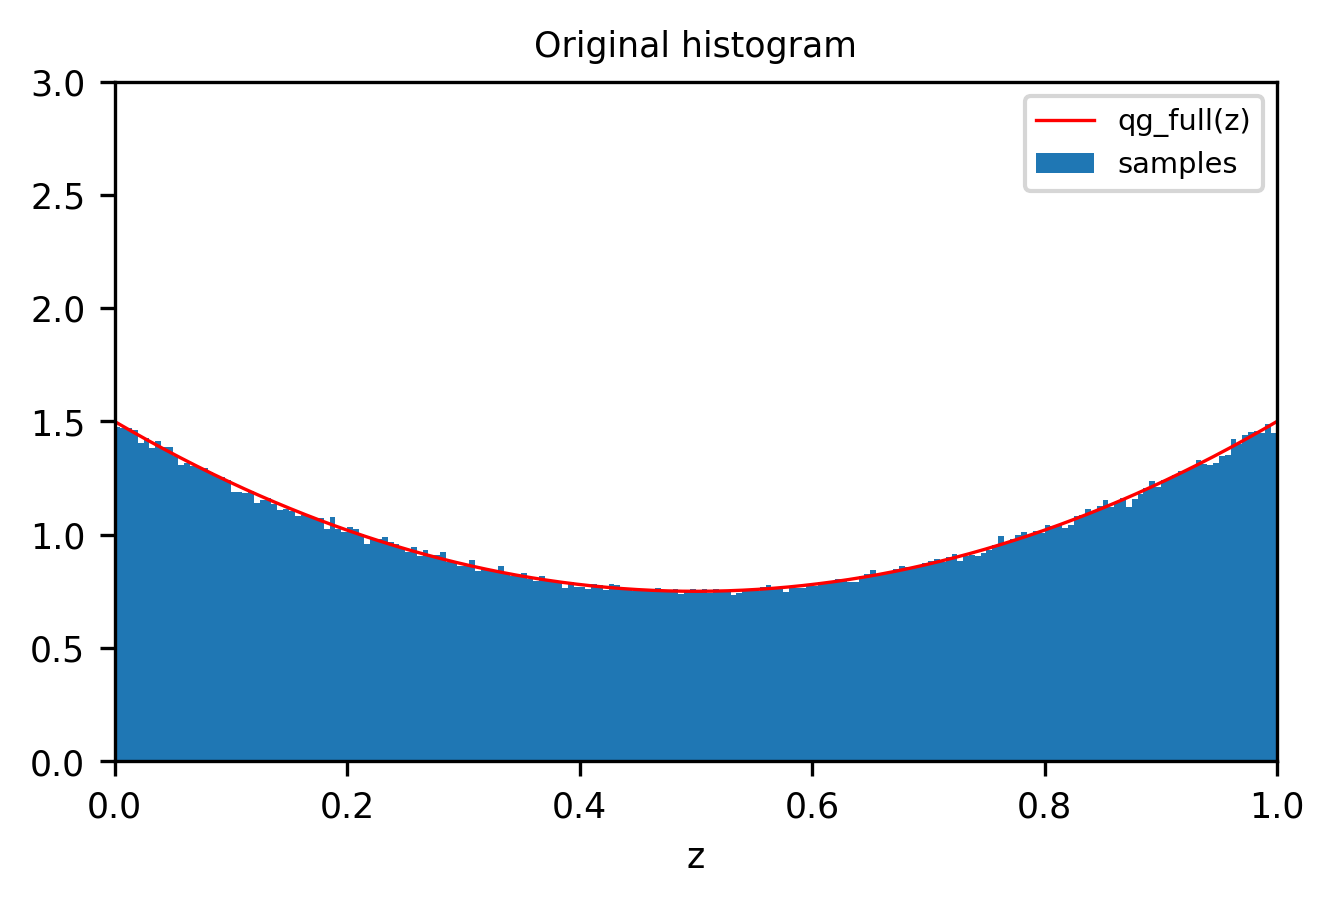
\includegraphics[width=9cm]{pictures/plots/Metropolis-Hastings/MH_vacuum_qg.png}
    \caption{Probability density of the full \(P_{qg}(z)\) splitting function, and the histogram of sampled values using \autoref{eqn: gqq_vacuum_sample}. Simulated with \(10^6\) samples.}
    \label{fig: p_qg_splitting}
\end{figure}

\subsubsection*{Sampling from the \(qq\) vertex}
Next up we will attempt to solve \autoref{eqn: energyfraction_function_R} for the \(P_{qq}(z)\) splitting function of \autoref{eqn: vacuum_qq_splitting_function}
\begin{align}
    \int dz\hat{P}_{qq}(z) &= \int \left(\frac{1+z^2}{1-z} \right)\, dz \nonumber \\
    %&= \int \left(\frac{-(z^2+1)}{z-1} \right)\, dz \nonumber \\
    %&= \int \left(\frac{-((z-1)(z-1)+2z)}{z-1} \right)\, dz \nonumber \\
    &= \int -(z-1)\, dz - \int \frac{2z}{z-1} \, dz \nonumber \\
    &= \int (1-z) \, dz - \int \frac{2(u+1)}{u} \, du \qquad \text{, where}\; u=z-1 \nonumber \\
    %&= \int (1-z) \, dz - \int 2\, dz - \int_a^b \frac{2}{u} \, du \nonumber  \\
    &= -\int (z+1) \, dz - \int \frac{2}{u} \, du \nonumber  \\
    &= -\frac{z^2}{2} - z - 2 \ln(z-1) 
\end{align}
since this integral has an exact solution, we can solve \autoref{eqn: energyfraction_function_R} for this splitting function:
\begin{align}
    %\mathcal{R}  \left[-\frac{z^2}{2} - z - 2\, \ln(z-1) \right]_\epsilon^{1-\epsilon} &= \left[-\frac{z^2}{2} - z - 2\, \ln(z-1) \right]_\epsilon^{y} \nonumber \\
    %\mathcal{R}  \left(-\frac{(1-\epsilon)^2}{2} - (1-\epsilon) - 2 (\ln((1-\epsilon)-1)) \right) &- \mathcal{R}  \left( -\frac{\epsilon^2}{2} - \epsilon - 2 (\ln(\epsilon-1)) \right) \nonumber \\
    %&= \left(-\frac{y^2}{2} - y - 2 (\ln(y-1)) \right) - \left( -\frac{\epsilon^2}{2} - \epsilon - 2 (\ln(\epsilon-1)) \right) \nonumber
    %\mathcal{R}|  \frac{6 \epsilon-3}{2} - 2\, \ln(-\epsilon) + 2\, \ln(\epsilon-1) &= -\frac{y^2}{2} - y - 2 \,\ln(y-1) +\frac{\epsilon^2}{2} + \epsilon + 2 \,\ln(\epsilon-1) \nonumber\\
    \frac{y^2}{2} + y + \ln \left( \frac{y-1}{\epsilon-1}\right)^2  &= -\left(\mathcal{R}  \frac{6 \epsilon-3}{2} + \frac{-\epsilon^2-4 \epsilon}{2}\right) -\ln\left(\frac{1-\epsilon}{\epsilon}\right)^{2\, \mathcal{R}}.
\end{align}
This equation is however difficult to solve, so we will need to use the Metropolis-Hastings algorithm once again. Attempting with a dummy function
\begin{align}
    %\int \left(\frac{-2}{z-1}\right)dz &= -2\,\ln(z-1) \\
    P_{qq}^{\text{dummy}}(z) &= \frac{-2}{z-1}
\end{align}
then \autoref{eqn: energyfraction_function_R} becomes
\begin{align}
    \mathcal{R} \left[-2\ln(z-1)\right]_{\epsilon}^{1-\epsilon} &= \left[-2\ln(z-1)\right]_{\epsilon}^{y} \nonumber \\
    \mathcal{R} \left(-2\ln((1-\epsilon)-1) + 2\ln(\epsilon-1) \right) &= \left(-2\ln(y-1) + 2\ln(\epsilon-1) \right) \nonumber \\
    \mathcal{R}\ln\left(\frac{1-\epsilon}{\epsilon} \right) &= -\ln(y-1) +\ln(\epsilon-1)
\end{align}
rearranging terms and exponentiating both sides 
\begin{align}\label{eqn: qq_sampling_y_function}
   \ln(y-1) &=\ln(\epsilon-1) -\ln\left(\frac{1-\epsilon}{\epsilon} \right)^{\mathcal{R}} \nonumber \\
    %y-1 &= \frac{e^{ln(\epsilon-1)}}{e^{ln(\frac{1-\epsilon}{\epsilon})^{\mathcal{R}}}} \nonumber \\
    y &= \frac{\epsilon-1}{(\frac{1-\epsilon}{\epsilon})^{\mathcal{R}}} +1 .
\end{align}
\autoref{eqn: qq_sampling_y_function} can be used for sampling random values from the simple \(qq\) splitting function, and following the same procedure as in Section \ref{sec: metropolis_hastings} we can implement Metropolis-Hastings algorithm for sampling random values from the full \(qq\) splitting function. The results of both the original samples, and the MH corrected histogram is given in \autoref{fig: MH_corrected_p_qq_splitting}.
\begin{figure}[htb]
    \centering
    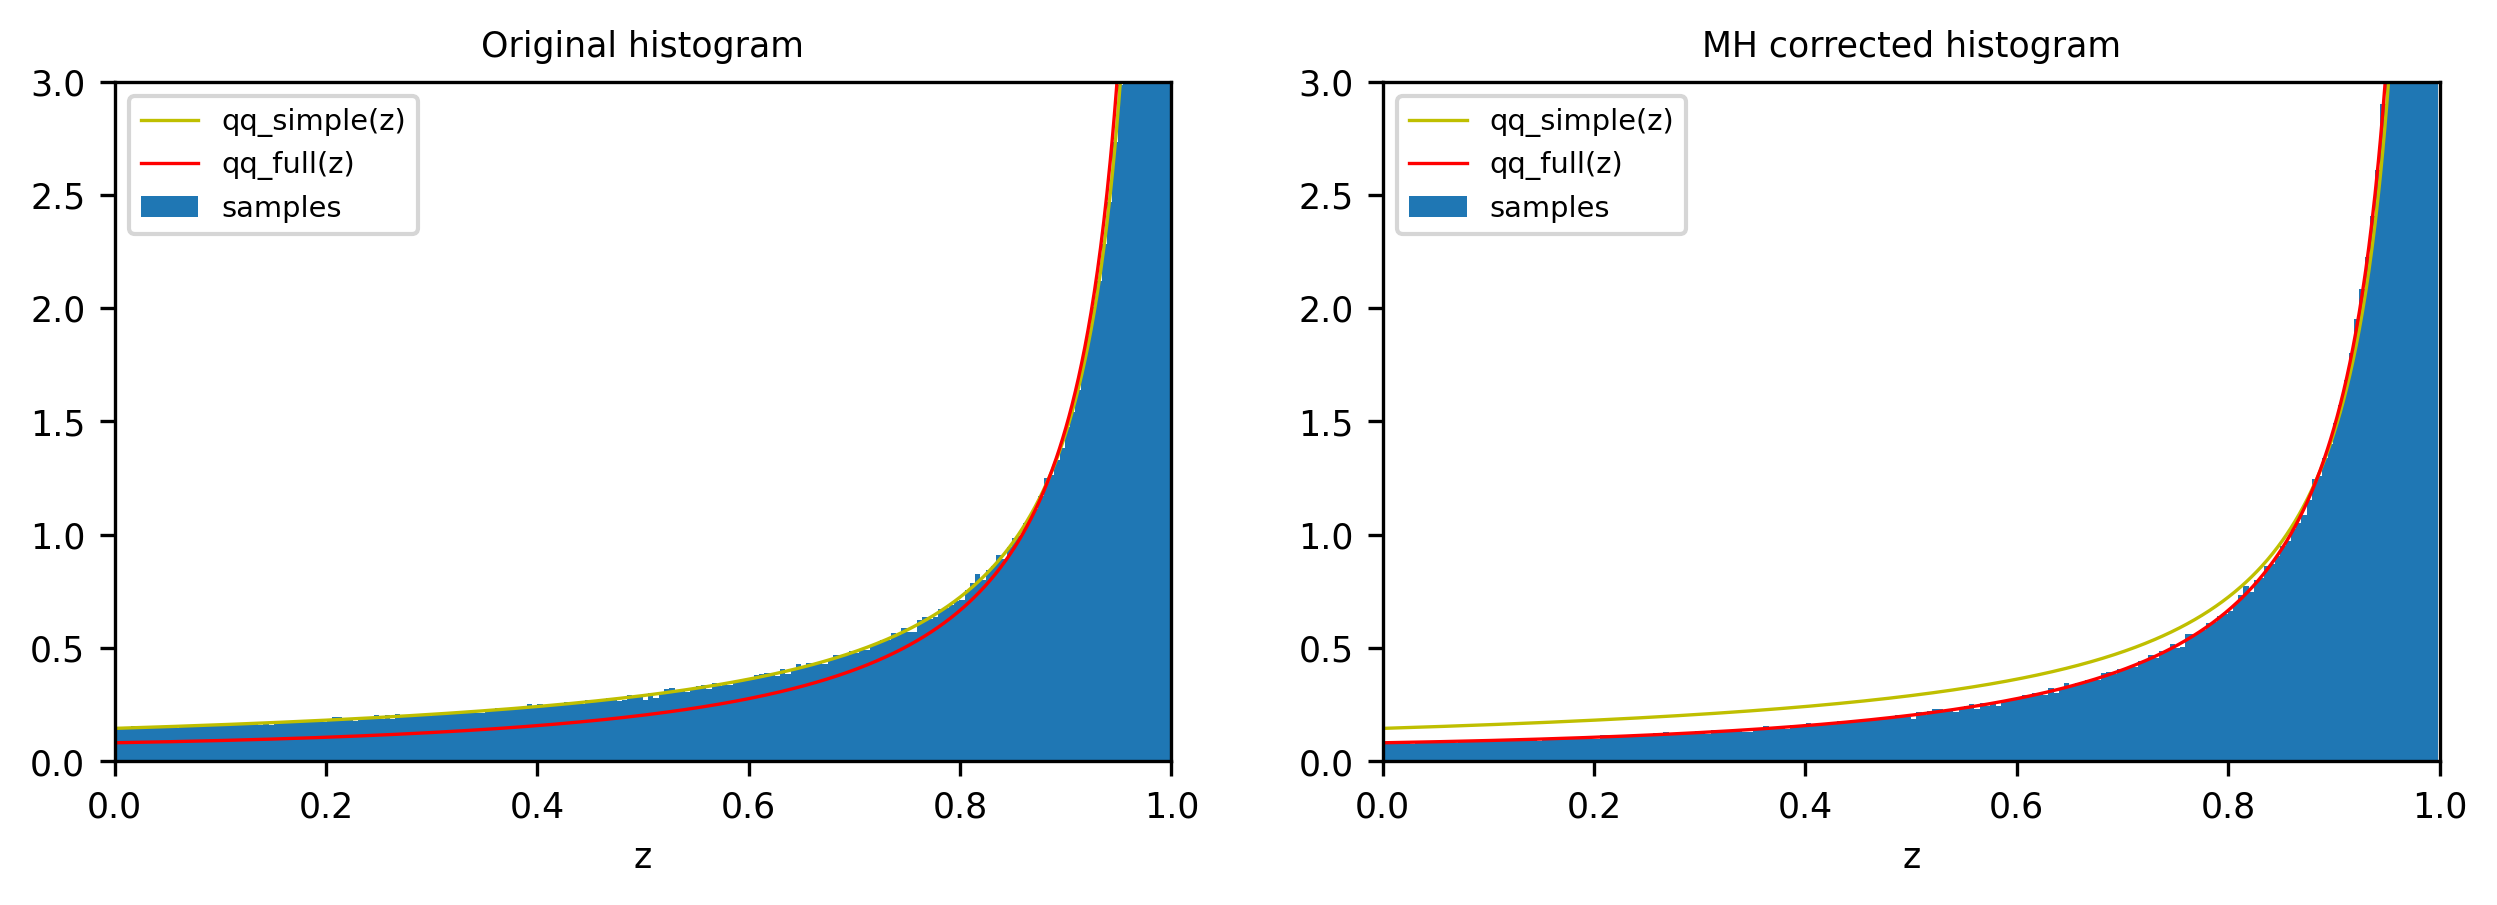
\includegraphics[width=15cm]{pictures/plots/Metropolis-Hastings/MH_vacuum_qq.png}
    \caption{Probability density of the full \(P_{qq}(z)\) splitting function and the dummy splitting function \(P_{qq}^{\text{dummy}}(z)\). The left plot gives the values sampled from \autoref{eqn: qq_sampling_y_function},and the right plot is corrected using Metropolis-Hastings algorithm. Simulated with \(10^6\) samples, and a MH acceptance rate of \(0.89\).}
    \label{fig: MH_corrected_p_qq_splitting}
\end{figure}

\subsection{Monte-Carlo implementation}\label{sec: MC_implementation_vacuum}
This section serves to give a brief overview of the logical structure of the main \textit{generate\_shower} subprogram, which is the core of the parton-shower programs. This is where all of the actual physics is applied, while the rest of the program is for plotting, defining variables, and managing parent/daughter relations.

The full code for running the different parton shower programs, and Metropolis-Hastings algorithms is available on the authors GitHub~\cite{GitHub_thesis}. The main loop running in the shower program is given here in \autoref{alg: generate_shower_loop}. Not all parameters are listed here, as to keep the representation as simple as possible.
\begin{center}
\begin{minipage}{.8\linewidth}
\begin{algorithm}[H]
\caption{generate\_shower main loop}
\label{alg: generate_shower_loop}
\begin{algorithmic}[1]
    \While{$ \text{len}(\text{SplittingPartons} > 0 $}
    \State SplittingParton, \(\Delta t\) = select\_splitting\_parton()
    \State \(t = t + \Delta t\)
    \State end\_shower = loop\_status(\(t, t_{\text{max}}\)) 
    \If{end\_shower}
        \State \textbf{break}
        \EndIf
    \State SplittingPartons.remove(SplittingParton)
    \State FinalList.remove(SplittingParton)
    \State $z$ = SplittingParton.split()
    
    \For{j \textbf{in} range(0,2)}
        \If{j==0}
            \State NewParton = Parton(\(t, xz\))
        \ElsIf{j==1}
            \State NewParton = Parton(\(t, x (1-z)\))
            \EndIf
            \EndFor
    \State Shower0.FinalList.append(NewParton)
    \If{NewParton.InitialFrac > \(z_{\text{min}}\sim 0.001\)}
        \State SplittingPartons.append(NewParton)
        \EndIf
    \EndWhile
    \State \textbf{return} Shower
\end{algorithmic}
\end{algorithm}
\end{minipage}
\end{center}

\subsection{Results for vacuum showers}
The mathematics and structure of the Monte-Carlo programs have now been presented, and we are therefore ready to examine the resulting distributions. For the vacuum programs, we are primarily interested in the inclusive parton, or inclusive energy distributions, given in terms of the momentum-fraction \(z_i\) of the different partons. 

\subsubsection*{Results for gluon showers in vacuum}
Starting by looking at the results for the parton shower with gluons in vacuum, where the inclusive energy distribution \(D(x,t)\) is generated using using the simplified splitting function \autoref{eqn: p_ggg_vacuum_dummy}. The results can be compared with the solution of the DGLAP equations which we obtained in \autoref{eqn: DGLAP_solution_energyflowmedium}, valid in the small \(x\) limit, the resulting plot is given in \autoref{fig: vacuum_gluons_MCandAnalytical_comparison_lin}.
\begin{figure}[htb]
    \centering
    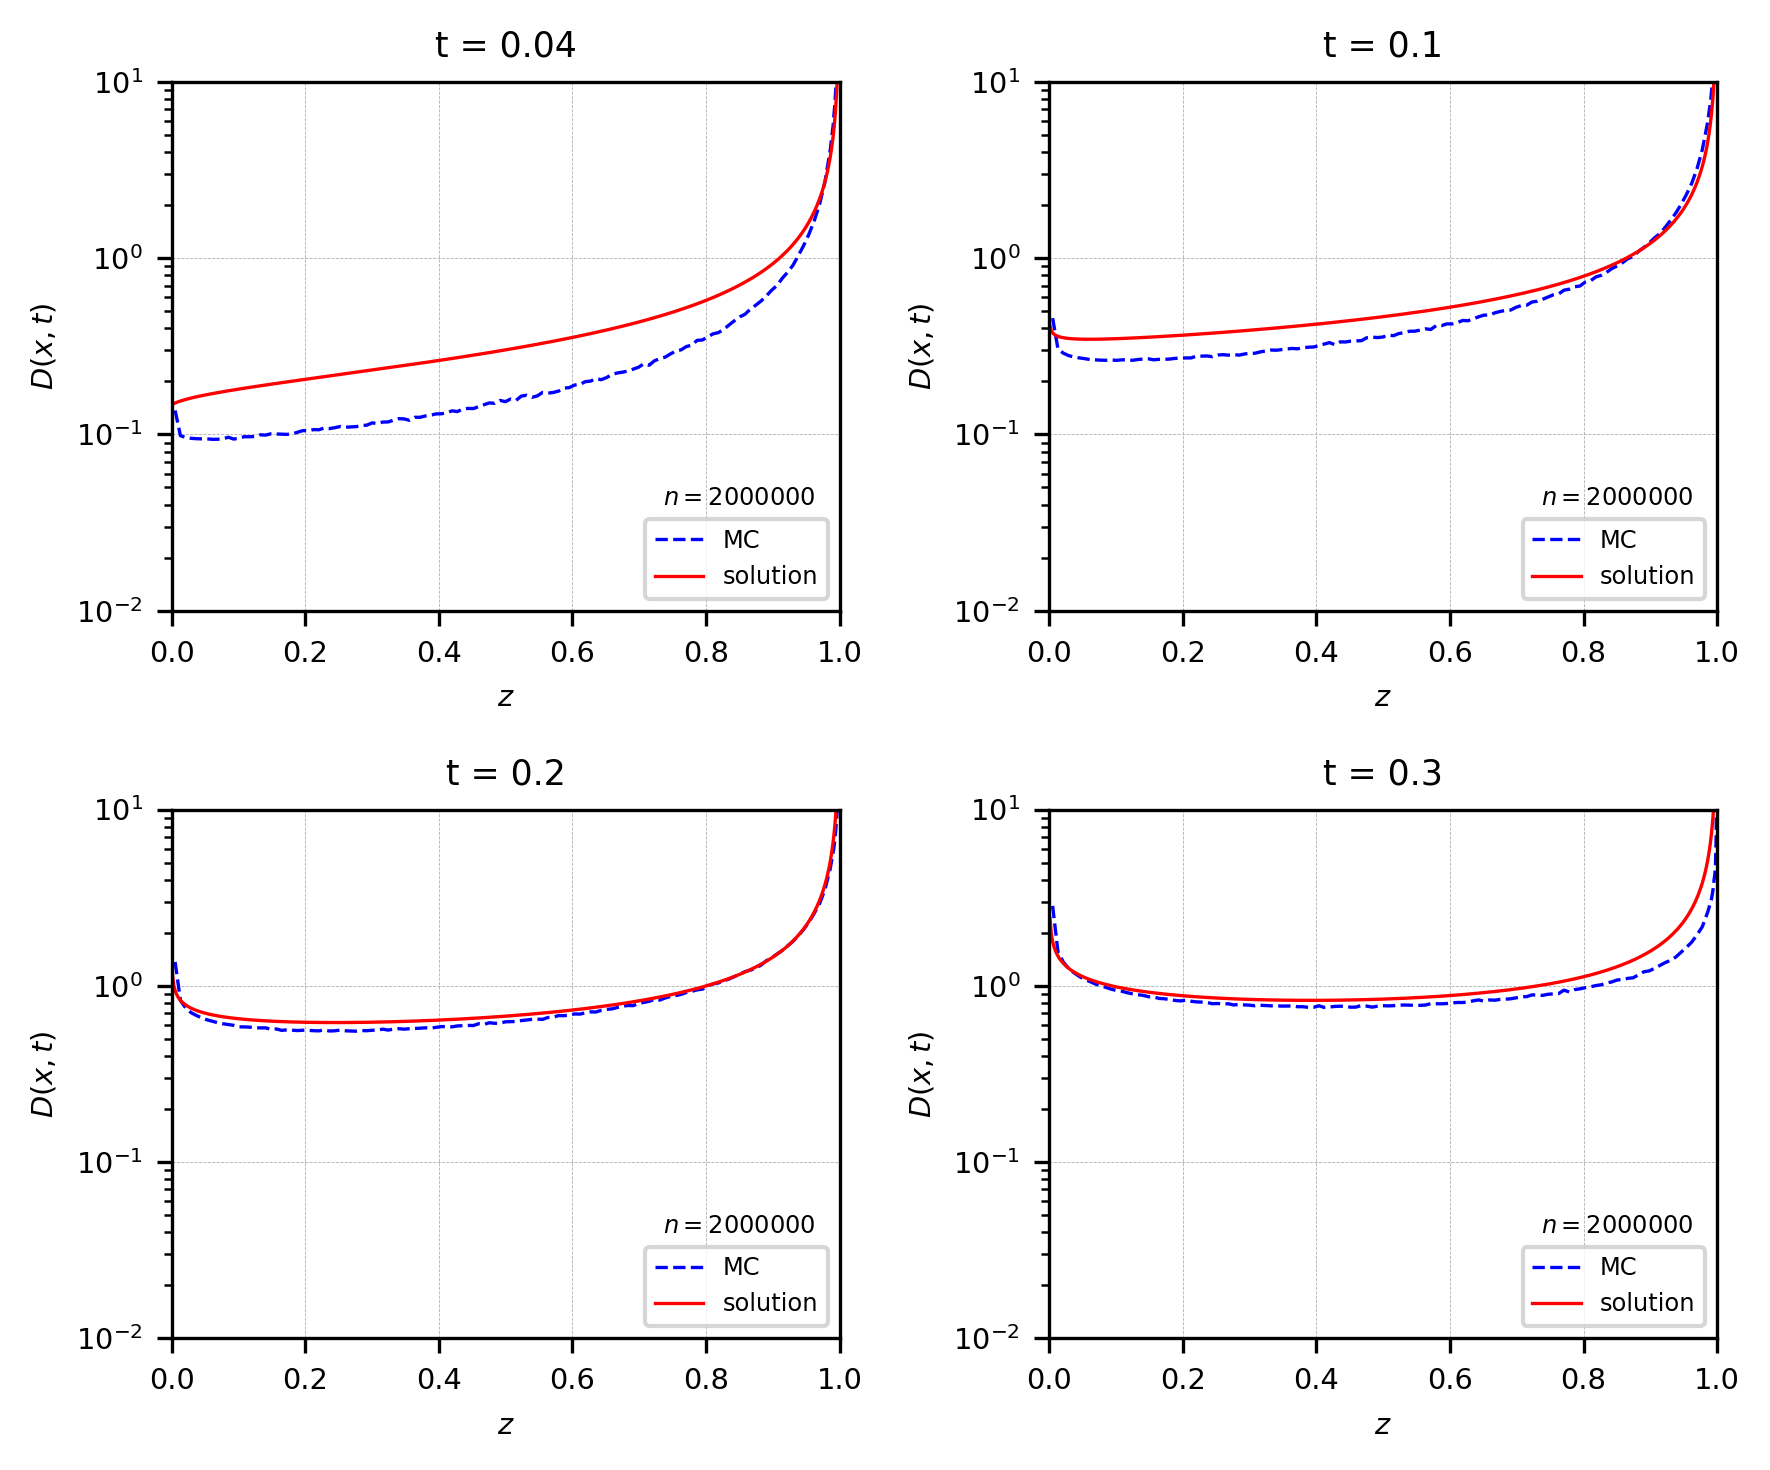
\includegraphics[width=13cm]{pictures/plots/distributions/vacuum/vacuum_shower_analytical_2m_lin.png}
    \caption{The inclusive energy distribution \(D(x,t)\) for gluon showers in vacuum. The red line is the analytical solution obtained in \autoref{eqn: DGLAP_solution_energyflowmedium}. The blue dotted line is the generated values by running \(n=2\cdot10^6\) showers in a Monte-Carlo program, using the dummy splitting function \autoref{eqn: p_ggg_vacuum_dummy}. Parameters used are \(\epsilon=10^{-3}\) and \(z_{\text{min}}=10^{-3}\)}.
    \label{fig: vacuum_gluons_MCandAnalytical_comparison_lin}
\end{figure}

The Monte-Carlo generated distribution plotted in \autoref{fig: vacuum_gluons_MCandAnalytical_comparison_lin} is in fairy good agreement with the analytical results for large values of the evolution variable \(t\), and small values of the momentum \(x\). This as expected as the solution is only valid for small values of \(x\) where \(\ln \frac{1}{x} >>t\).

\subsubsection*{Results for quarks-, and gluons showers in vacuum}
Turning to the Monte-Carlo for both quarks and gluons in vacuum, generated using the full splitting functions and sampled using the Metropolis-Hastings algorithm. This time there is no analytical results to compare with, but we can compare the inclusive parton distributions \(f(x,t)\), of quark-initiated and gluon-initiated showers. The resulting plot is given in \autoref{fig: vacuum_distribution_quark_and_gluon}. The final distributions contains both quarks and gluons, and the difference between them is simply the type of the initial parton. The hardest parton of each shower is also plotted using dotted lines, and it is simply determined by taking the parton with the highest momentum once the shower has terminated, and plotting its \(z\) value.
\begin{figure}[htb]
    \centering
    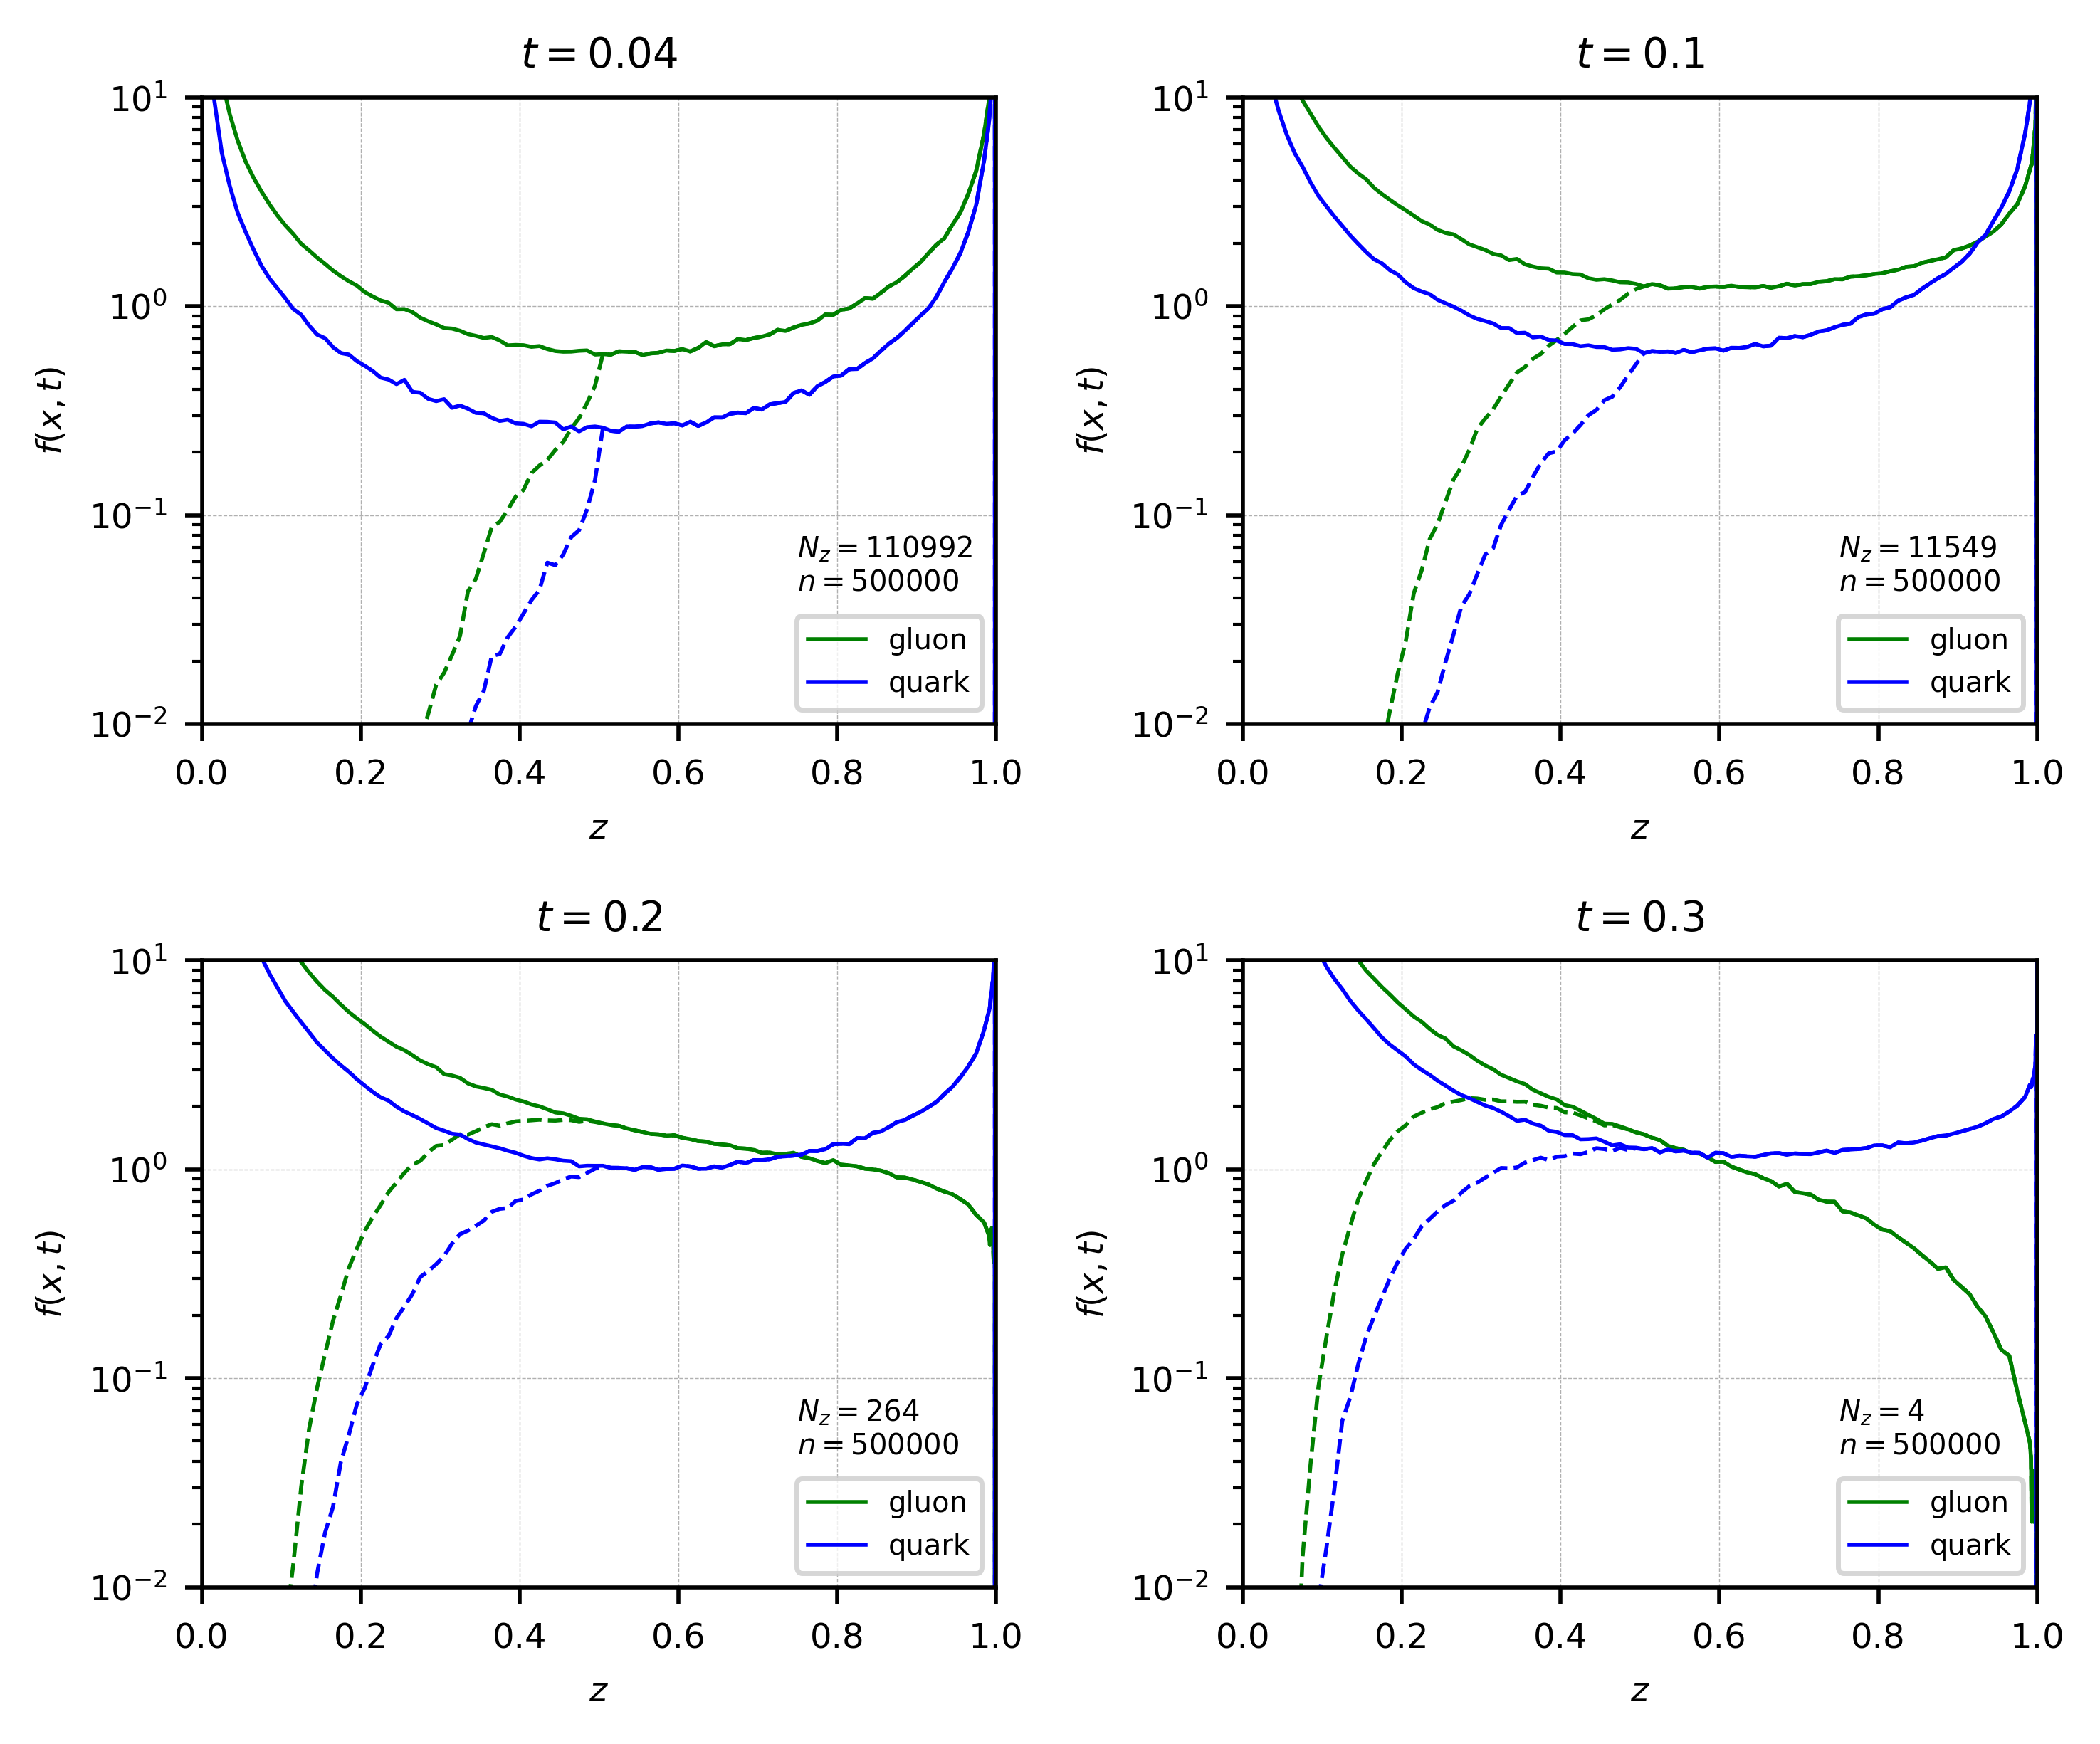
\includegraphics[width=13cm]{pictures/plots/distributions/vacuum/dasgupta_quarksgluons_N500000.png}
    \caption{The inclusive parton distribution \(f_i(x,t)\) for quarks and gluons in vacuum, generated by the Monte-Carlo program with both quarks and gluons in vacuum, using the full splitting functions. The solid lines show the inclusive parton distribution for initial quarks (blue) and initial gluons (green). The dashed lines show the hardest parton of each shower. Simulated with \(n=5\cdot10^5\) showers for both initial quark and initial gluon. Parameters used are \(\epsilon=10^{-3}\) and \(z_{\text{min}}=10^{-3}\). The number of gluons \(N_z\) with \(z=1\) is printed on each of the plots.}
    \label{fig: vacuum_distribution_quark_and_gluon}
\end{figure}

There are several observations to be made from \autoref{fig: vacuum_distribution_quark_and_gluon}. Firstly the distribution of the hardest parton of each shower is the same as the inclusive distribution for values above \(z<\frac{1}{2}\). This will be explored in more detail when we discuss leading partons in \autoref{cpt:leading}. Secondly, the impact the initial parton has on the distribution is significant, this is related to the expected branching intervals, and we will discuss it shortly.

An initial check of the validity of the program can be done by comparing with the results of~\cite[Figure 2.]{Dasgupta_2015}, in which the inclusive distribution has been plotted for fixed values of the evolution variable, \(t=0.04, 0.1, 0.2, 0.3\). While~\cite{Dasgupta_2015} discusses a slightly different approach, where the evolution goes from \(R<\theta<1\), meaning they obtain the total number of microjets within a given jet, as opposed to our treatment where we are looking for the parton distribution inside a jet with radius \(R\) such that, \(Q_0/p_t < \theta < R\). The result can however be compared as long as the evolution goes over the same effective angle, as is the case when we are plotting with the same values of \(t\). Our results are therefore in good agreement with~\cite{Dasgupta_2015}.

More explicit calculations can be done for checking the validity of our results. From the DGLAP equation on integral form \autoref{eqn: DGLAP_evolutioneq_unregularized_integral_ellis}, there is a term \(\Delta(t)\, f(x,t_0)\), which represents the probability of no branching to occur at all for the initial parton during the interval \(t\in[t_0, t_{max}]\). This can be calculated from \autoref{eqn: branching_probability_from_sudakov_gg} for initial gluons, except now we know the value of \(\Delta t\), and need to take into account the possibility of the gluon to branch into a \(gg\)-pair or a \(q\bar q\)-pair. The probability is then given as
\begin{equation}
    \mathcal{P}(t) = \exp \left(-t\, \int_{\epsilon}^{1-\epsilon}dz\, (P_{gg}(z) + P_{qg}(z)) \right).
\end{equation}
Using the same values for \(t\) and \(\epsilon\) as in the plot:
\begin{align}\label{eqn: no_branching_sudakov_probability}
    \begin{split}
        \mathcal{P}(0.04) &\approx 2.22\cdot 10^{-1} \\
        \mathcal{P}(0.1) &\approx 2.32\cdot 10^{-2} \\
        \mathcal{P}(0.2)&\approx 5.40\cdot 10^{-4} \\
        \mathcal{P}(0.3) &\approx 1.25\cdot 10^{-5}.
    \end{split}
\end{align}
These probabilities should manifest themselves in our plot, and we can find them by simply counting the number of partons \(N_z\) with momentum \(z=1\) in the final distribution for each value of \(t\). The values for \(N_z\) is given in \autoref{fig: vacuum_distribution_quark_and_gluon}, and correspond to the following probabilites:
\begin{align}\label{eqn: no_branching_MC_probability}
    \begin{split}
        \mathcal{P}_{\text{MC}}(t=0.04) &= \frac{N_z(0.04)}{N} = \frac{110992}{5 10^{5}} \approx 2.22 \cdot10^{-1} \\
        \mathcal{P}_{\text{MC}}(t=0.1) &= \frac{N_z(0.1)}{N} = \frac{11549}{5 10^{5}} \approx 2.31\cdot 10^{-2} \\
        \mathcal{P}_{\text{MC}}(t=0.2) &= \frac{N_z(0.2)}{N} = \frac{264}{5 10^{5}} \approx 5.28\cdot 10^{-4} \\
        \mathcal{P}_{\text{MC}}(t=0.3) &= \frac{N_z(0.3)}{N} = \frac{4}{5 10^{5}} \approx 8\cdot 10^{-6}.
    \end{split}
\end{align}
We can see that the probabilities given from the calculation of the Sudakov in \autoref{eqn: no_branching_sudakov_probability} is in reasonable good agreement with the probabilities we find when running \(5 \cdot 10^5\) showers and counting \(N_z\) in \autoref{eqn: no_branching_MC_probability} - which should be expected as the Sudakov form factor is used both for the calculation, and in the Monte-Carlo.

It could be argued that the results generated by the quarks and gluons cascade are more accurate than the gluon cascade, as there is no reason for a gluon not to branch into a \(q\bar q\)-pair\footnote{It is however significantly less likely for than \(g\rightarrow gg\) branchings, for our program about \(\sim 4\%\) of the gluon branchings are \(g\rightarrow q\bar q\)}. It would therefore be interesting to compare the distribution of the pure gluon shower in vacuum as given in \autoref{fig: vacuum_gluons_MCandAnalytical_comparison_lin}, with the showers initiated by a gluon as given in \autoref{fig: vacuum_distribution_quark_and_gluon}. The resulting plot is given in \autoref{fig: vacuum_program_comparisons}.
\begin{figure}[htb]
    \centering
    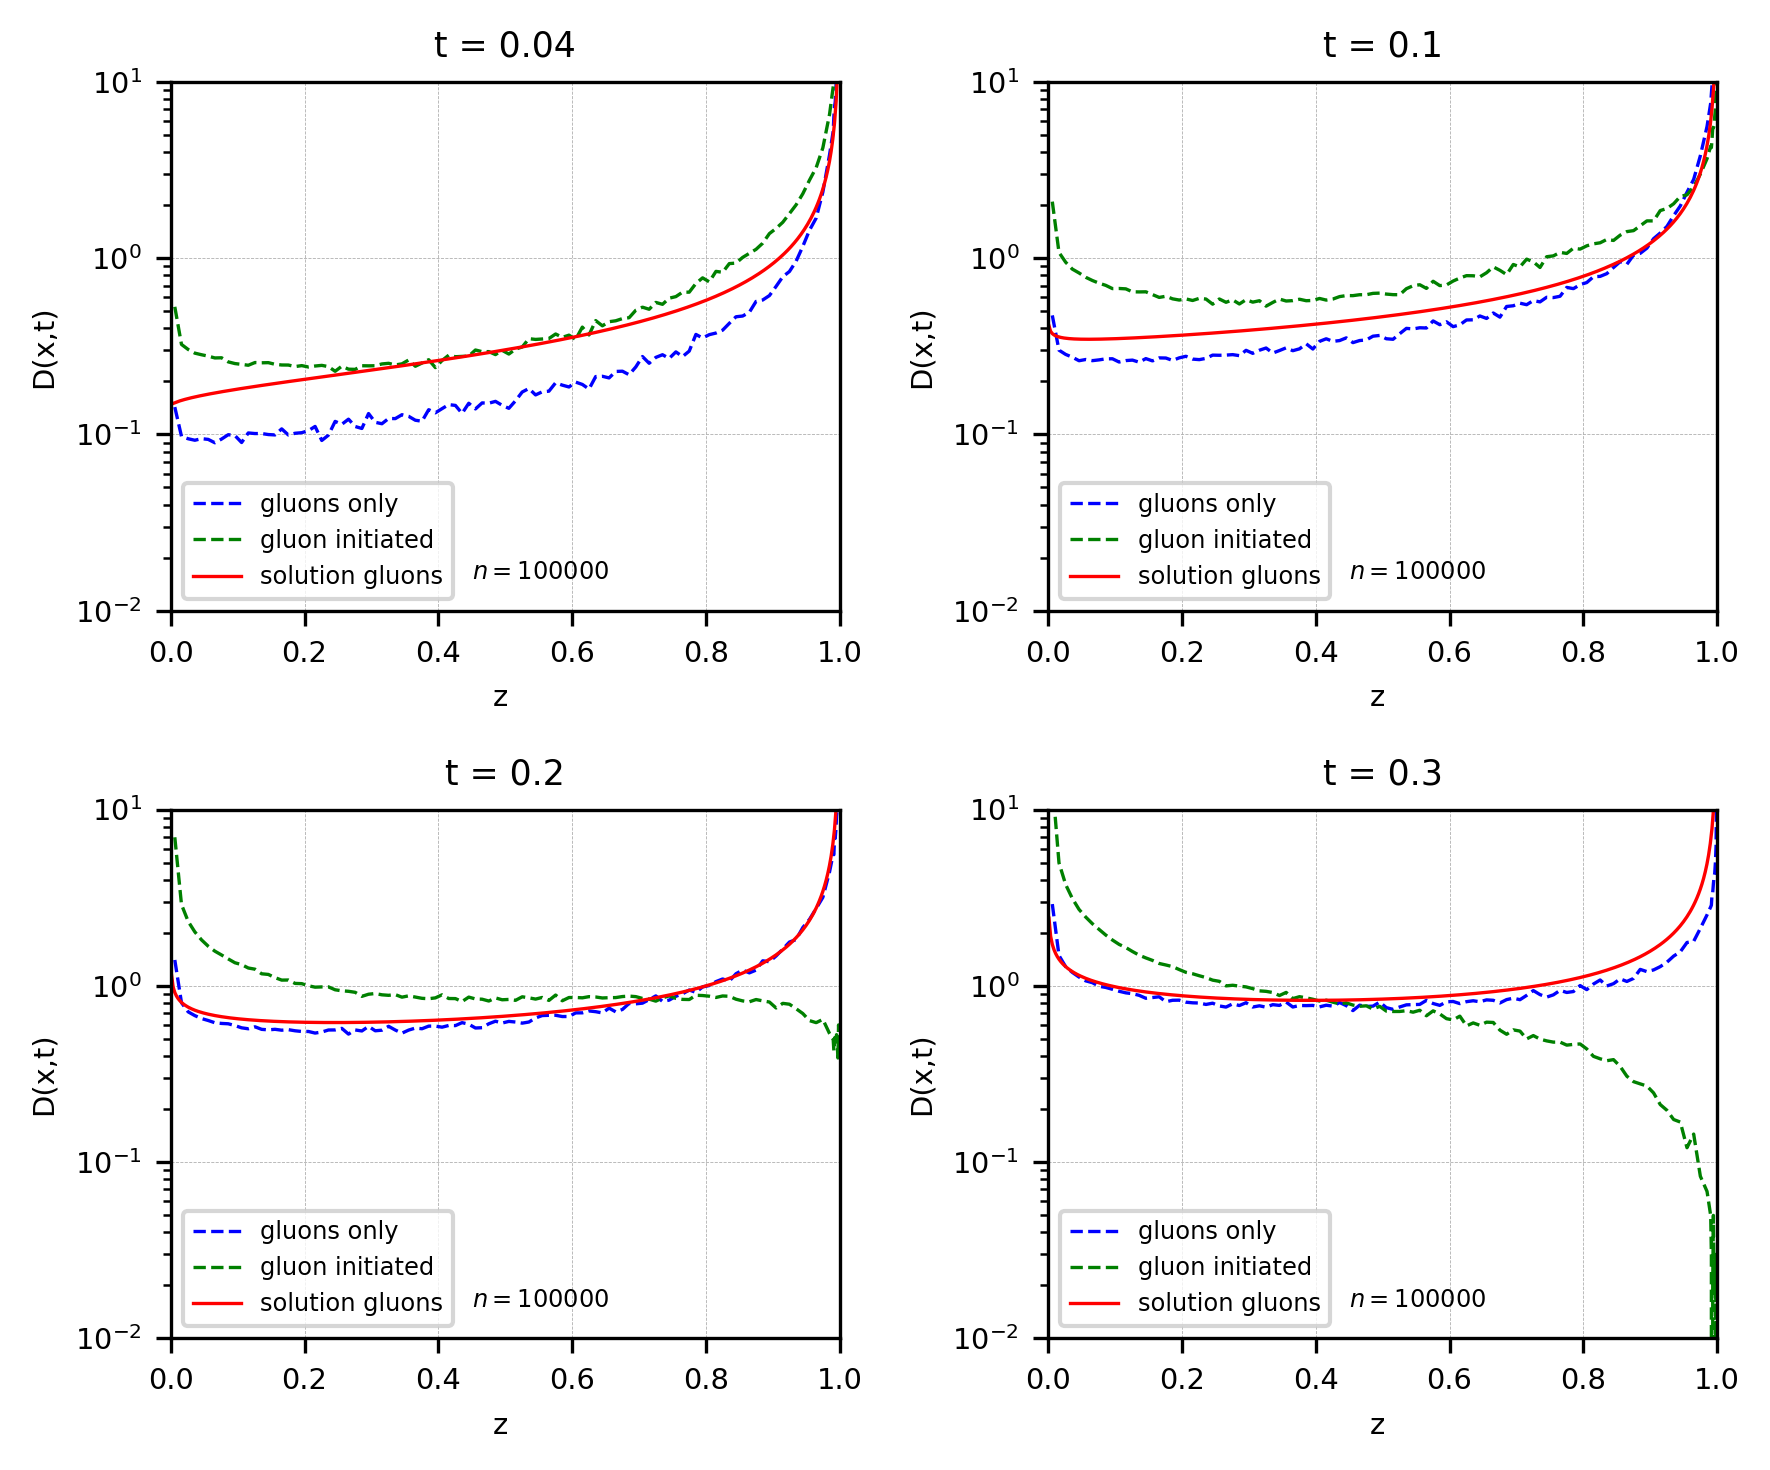
\includegraphics[width=13cm]{pictures/plots/distributions/program_comparison/comparison_vacuum_programs_100k_lin.png}
    \caption{The inclusive energy distribution \(D(x,t)\) generated by both Monte-Carlo programs: gluons in vacuum (blue), and quarks-and-gluons in vacuum, initiated by a gluon(green). The red line is the analytical solution of the DGLAP equation obtained in \autoref{eqn: DGLAP_solution_energyflowmedium} for gluons, which is only valid in the small \(x\) and large \(t\) limits. Simulated with \(n = 10^5\) showers, using \(\epsilon=10^{-3}\) and \(z_{\text{min}}=10^{-3}\).}
    \label{fig: vacuum_program_comparisons}
\end{figure}

The plot given here is a straight-up comparison of the two programs. It is therefore important to note that the splitting functions are not identical as the gluon showers is using the simplified splitting function which does not carry any color factors. This is apparent when examining the integrals over the different splitting functions, using \(\epsilon = 10{-3}\):
\begin{align}
\begin{split}
    \int_\epsilon^{1-\epsilon} P_{gg}^{\text{simple}}(z)\,dz &\approx 13.8\\ \int_\epsilon^{1-\epsilon} P_{gg}(z)\,dz &\approx 36.0\\ 
    \int_\epsilon^{1-\epsilon} P_{qg}(z)\,dz &\approx 1.7 \\
    \int_\epsilon^{1-\epsilon} P_{qq}(z)\,dz &\approx 16.4.
\end{split}
\end{align}
Since the expected splitting intervals are inversely proportional to these integrals, it is to be expected that the gluon showers using the simplified \(P_{gg}^{\text{simple}}\) splitting function, would be going slower toward small momentum values. If we were to adjust the simplified splitting function such that the expected intervals of \(gg\) branchings were identical, then the gluon-only distribution would go faster towards low momentum values than the gluon initiated showers with both quarks and gluons. 

There are two reasons for this. The first is that gluons can split using either the \(P_{gg}(z)\) or \(P_{qg}(z)\) splitting function, the second is that when we inevitably observe a \(qg\) splitting, those new quarks will split much slower than gluons. Both of these properties are direct consequences of how the branching intervals are calculated. We can check for this behavior by simply adding a fictitious color factor \(C\sim 2.6\) to the simplified splitting function such that
\begin{equation}
    \int_\epsilon^{1-\epsilon} C P_{gg}^{\text{simple}}(z) dz \approx \int_\epsilon^{1-\epsilon} P_{gg}(z) dz.
\end{equation}
The two distributions with this new factor is given in \autoref{fig: vacuum_program_comparisons_Cfictitious}. It is now apparent that the gluon showers is going faster towards small momentum values, as there are no quarks to slow down the splitting process. The difference in color factors does not affect the splitting values in the same manner, as those are calculated by two integrals over the splitting function, meaning the constant factors simply cancel each other out.
\begin{figure}[hbt]
    \centering
    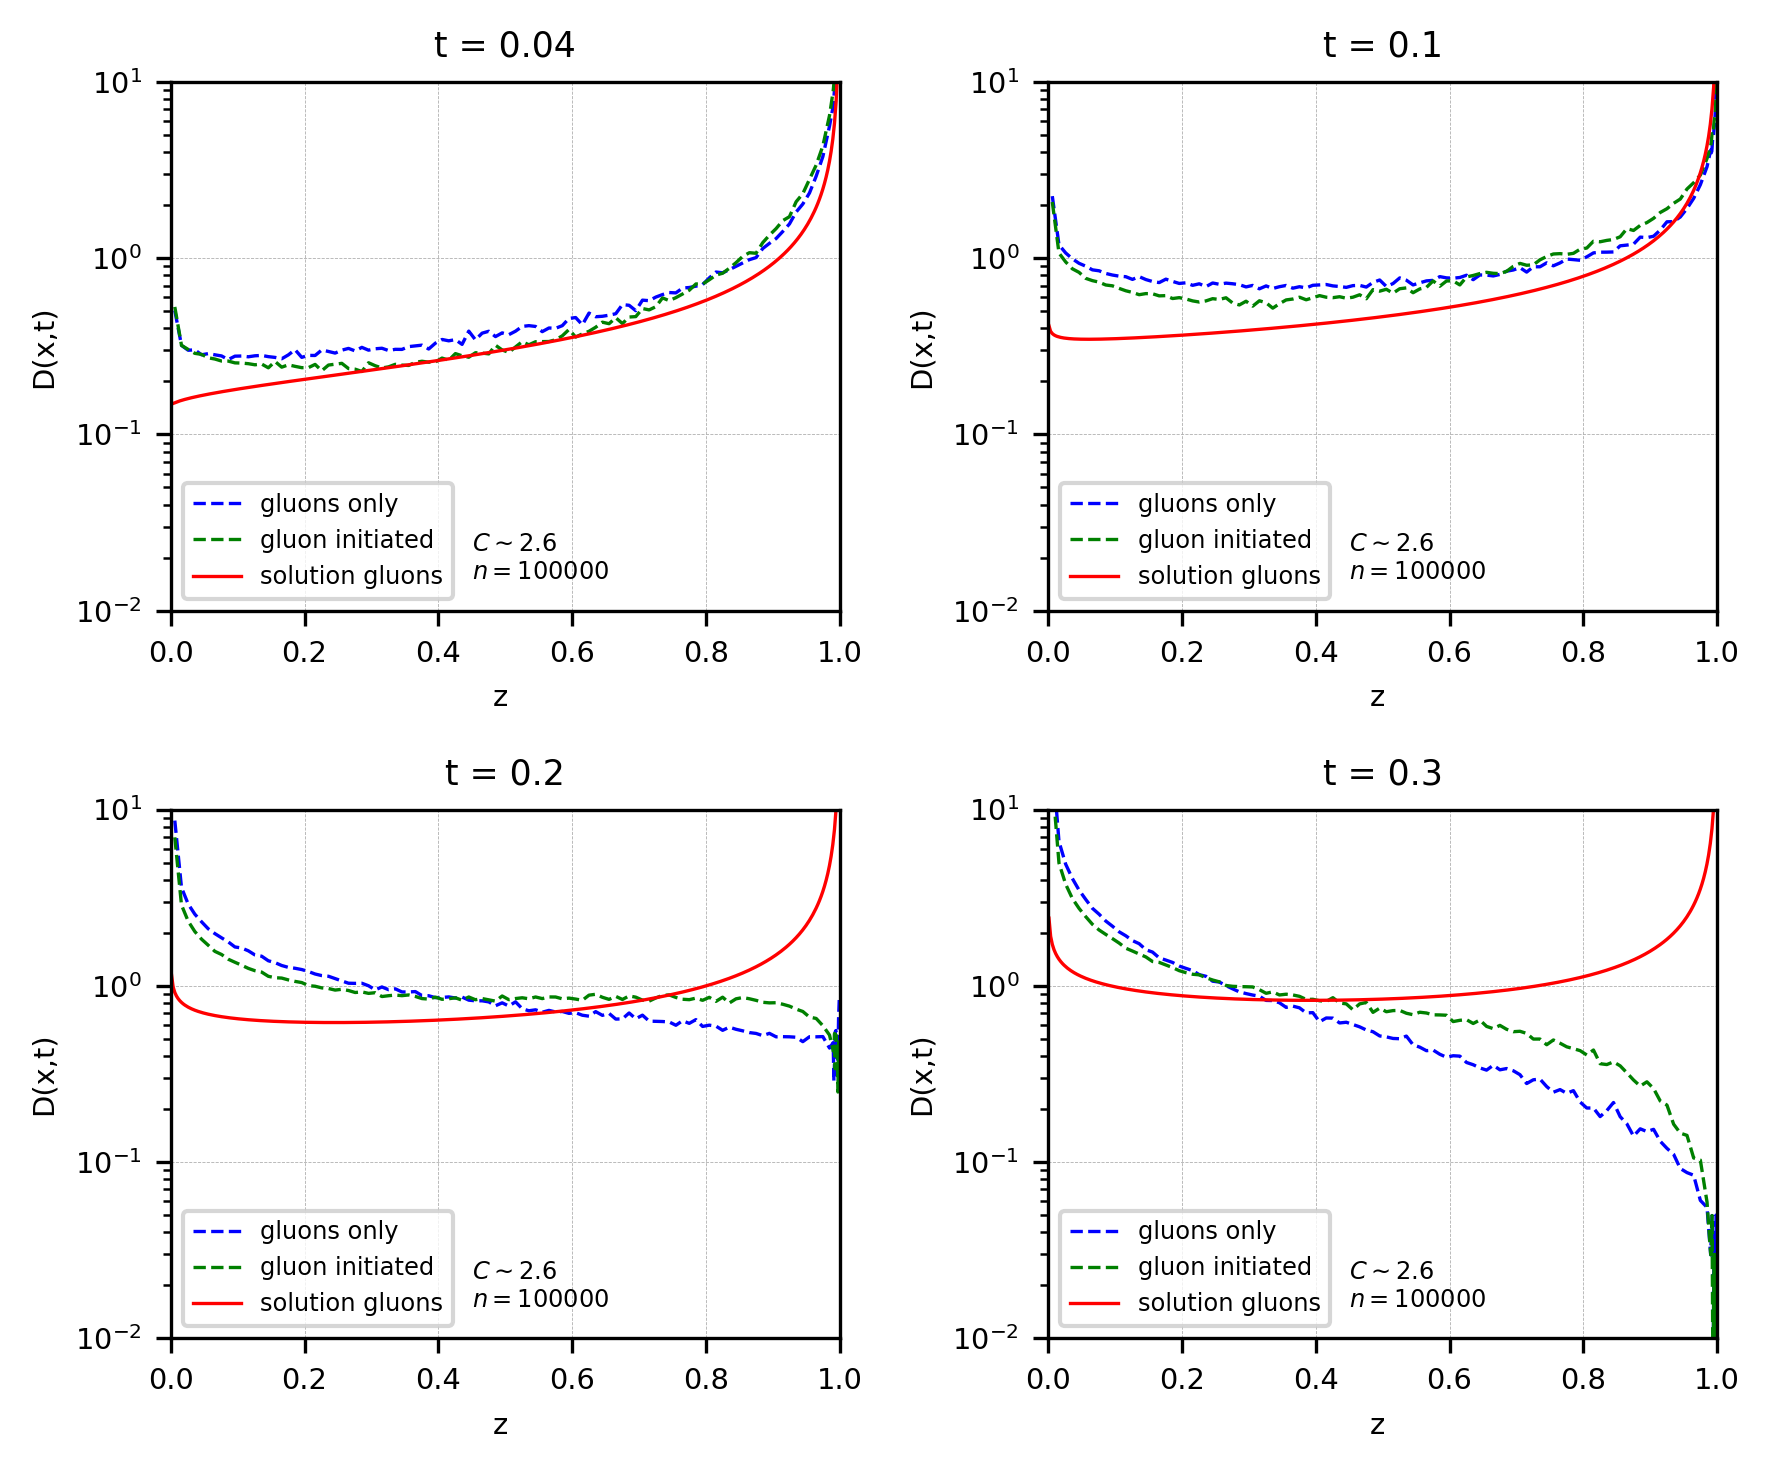
\includegraphics[width=13cm]{pictures/plots/distributions/program_comparison/comparison_vacuum_programs_100k_lin_cfact.png}
    \caption{The inclusive energy distribution \(D(x,t)\) generated by both Monte-Carlo programs. Blue: gluons in vacuum, but with a fictitious color factor \(C\sim2.6\) added to the simplified splitting function such that the expected branching interval of gluons are the same. Green: quarks-and-gluons in vacuum, initiated by a gluon. The red line is the analytical solution of the DGLAP equation obtained in \autoref{eqn: DGLAP_solution_energyflowmedium} for gluons, which is only valid for gluons and in the small \(x\) and large \(t\) limits. Simulated with \(n = 10^5\) showers, using \(\epsilon=10^{-3}\) and \(z_{\text{min}}=10^{-3}\).}
    \label{fig: vacuum_program_comparisons_Cfictitious}
\end{figure}

\subsubsection*{Validity of our Monte-Carlo in vacuum}
The Monte-Carlo programs developed for vacuum cascades has now been under scrutiny, so lets quickly summarize the findings. 
\begin{enumerate}
    \item The results of the Monte-Carlo gluon cascade was compared with the analytical solution calculated in \autoref{sec: solution_DGLAP} and was in good agreement in the small \(x\) large \(t\) limit, as expected. 
    \item The inclusive distribution generated by gluon-initiated and quark-initiated showers, was visually compared with the results presented in~\cite{Dasgupta_2015}, and we can see that the results were visually identical.
    \item The number of initial partons which do not branch in the interval \([t_{\text{min}}, t_{\text{max}}]\) was calculated from the Sudakov form factor for initial gluons, and compared with the Monte-Carlo for quarks and gluons. The numbers were of similar order.
    \item The behaviour of the gluon cascade was compared with the quarks and gluons cascade. This was done by highlighting how adjusting for the expected branching intervals, still yielded different distributions. This was attributed to the addition of quarks in the shower, which generally makes it go slower towards small values.
\end{enumerate}
While no formal comparison has been done with the results of well established event generators such as PYTHIA~\cite{PYTHIA_Bierlich:2022pfr}, the discussion presented here should spark confidence in our simple parton shower generator.
 

\clearpage
\section{Monte-Carlo for Parton Branching in Medium}
When developing a Monte-Carlo program for medium cascades, we will be restricting ourselves to gluons in medium, and use the simplified medium splitting function, or reduced kernel. This is done such that we can compare our results with the analytical solution for the in-medium kinetic rate equation, and examine the properties of leading-parton cascades. The process of creating a parton shower program for both quarks and gluons in medium, would follow the same structure as in the previous section, but we will limit ourselves to gluons in this thesis.

\subsection{Evolution interval}
As discussed in \autoref{sec: BDMPS_theory}, the medium cascade evolves according to the actual time, and the characteristic time is simply the time it takes for the initial parton to radiate most of its energy into soft gluons. We will be evolving the cascades using the variable \(\tau = t/t_*\), which was defined in \autoref{eqn: medium_tau_definiton}. It is therefore not a hard cutoff for the medium cascade but serves more as an indication of how long the cascades can evolve, and it is an important property that will affect our expectations for different values of \(\tau\). There is therefore no upper limit on the value of \(\tau\) in our medium evolutions, but since most of the energy has disappeared into soft gluons \((z<0,001)\) at \(\tau \sim 1\), we might as well set this as an approximate boundary,
\begin{align}\label{eqn: medium_evolution_boundaries}
    0 < \tau &\lessapprox 1.
\end{align}
Determining the probable branching interval \(\Delta t\) can again be done from the Sudakov form factor, introduced for the medium evolution in \autoref{eqn: BDMPS_sudakov}, following the procedure presented in \autoref{sec: determining_evolution_time_from_sudakov}. Doing this in terms of \(\tau\), such that \(\Delta \tau = \Delta t/t_*\), and \(\Delta t/t_*(x) = \Delta t/t_* \sqrt{x} = \Delta \tau/\sqrt{x}\), the evolution probability takes the form
\begin{align}
    \mathcal{P}(\Delta \tau) &= \frac{\Delta(\tau_0)}{\Delta(\tau)} = \exp \left(- \frac{\Delta \tau}{\sqrt{x}} \int_\epsilon^{1-\epsilon} \, dz\, z \mathcal{K}(z) \right).
\end{align}
Exchanging the probability with a randomly generated number \(\mathcal{R}\in (0,1)\)
\begin{align}
    \Delta \tau &= -\frac{\sqrt{x}\,\ln(\mathcal{R}) }{\int_\epsilon^{1-\epsilon} \, dz\, z \mathcal{K}(z)}
\end{align}
and from the symmetry of the reduced kernel, we have \(\int_0^1 \, dz\, z \mathcal{K}(z) = \frac{1}{2} \int_0^1 \, dz \mathcal{K}(z)\), and the probable evolution interval an therefore be written as
\begin{equation}\label{eqn: BDMPS_probable_branching_interval_tau}
    \Delta \tau = -\frac{2\, \sqrt{x} \ln(\mathcal{R}) }{\int_\epsilon^{1-\epsilon} \, dz \mathcal{K}(z)}.
\end{equation}

\subsection{Sampling from the medium splitting function}
The full medium splitting functions was introduced in \autoref{sec: medium_splitting_functions} but it will be sufficient for our treatment of medium showers to use the reduced \(\mathcal{K}_{gg}(z)\) splitting kernel, as given in \autoref{eqn: ggg_medium_reduced_kernel}. A way of sampling the full splitting functions is available for the interested reader in \autoref{app: medium_MetropolisHastings}. 

\subsubsection*{Sampling from the reduced kernel}
Sampling from the reduced kernel presented in \autoref{eqn: ggg_medium_reduced_kernel} follows the same procedure as when sampling the vacuum splitting functions where we solved \autoref{eqn: energyfraction_function_R}. The integral of the reduced kernel is
\begin{align}
    \int_a^b \frac{1}{(z(1-z))^{3/2}}dz &= \left[ \frac{4z-2}{\sqrt{-z(z-1)}} \right]_a^b
\end{align}
and \autoref{eqn: energyfraction_function_R} is then
\begin{align}
    \mathcal{R} \int_\epsilon^{1-\epsilon} dz \, \frac{1}{(z(1-z))^{3/2}} &= \int_\epsilon^{y} \frac{1}{(z(1-z))^{3/2}} \nonumber \\
    %\mathcal{R} \left(  \frac{4(1-\epsilon)-2}{\sqrt{-(1-\epsilon)((1-\epsilon)-1)}} - \frac{4\epsilon-2}{\sqrt{-\epsilon(\epsilon-1)}} \right) &= \frac{4y-2}{\sqrt{-y(y-1)}} - \frac{4\epsilon-2}{\sqrt{-\epsilon(\epsilon-1)}} \nonumber\\
    \mathcal{R} \left(  \frac{2-4\epsilon}{\sqrt{\epsilon(1-\epsilon)}} - \frac{4\epsilon-2}{\sqrt{\epsilon(1-\epsilon)}} \right) &= \frac{4y-2}{\sqrt{-y(y-1)}} - \frac{4\epsilon-2}{\sqrt{-\epsilon(\epsilon-1)}} \nonumber\\
    \mathcal{R} \left(  \frac{4-8\epsilon}{\sqrt{\epsilon(1-\epsilon)}} \right) - \frac{2-4\epsilon}{\sqrt{\epsilon(1-\epsilon)}} &= \frac{4y-2}{\sqrt{-y(y-1)}}.
\end{align}
The term on the l.h.s can be written in terms of the integral again and assigned to a variable \(a\)
\begin{equation}
    a = \int_\epsilon^{1-\epsilon} dz  \left(\mathcal{R} - \frac{1}{2} \right) = \mathcal{R} \left(  \frac{4-8\epsilon}{\sqrt{\epsilon(1-\epsilon)}} \right) + \frac{2-4\epsilon}{\sqrt{\epsilon(1-\epsilon)}}
\end{equation}
using this \(a\), the remainder of the equation can be solved using Mathematica
\begin{align}\label{eqn: medium_gg_sampling}
    y &= \frac{16 + a^2 \mp a \sqrt{16 + a^2}}{2 (16 + a^2)} \nonumber\\
    y &= \frac{1}{2} \mp \frac{a \sqrt{16 + a^2}}{2 (16 + a^2)} \nonumber\\
    y &= \frac{1}{2} \mp \frac{a }{2 \sqrt{16 + a^2}}.
\end{align}
And we now have a method for randomly sampling from the reduced kernel. The histogram of the randomly sampled values compared to the exact splitting function is given in \autoref{fig: medium_gg_sampling}. 
\begin{figure}[htb]
    \centering
    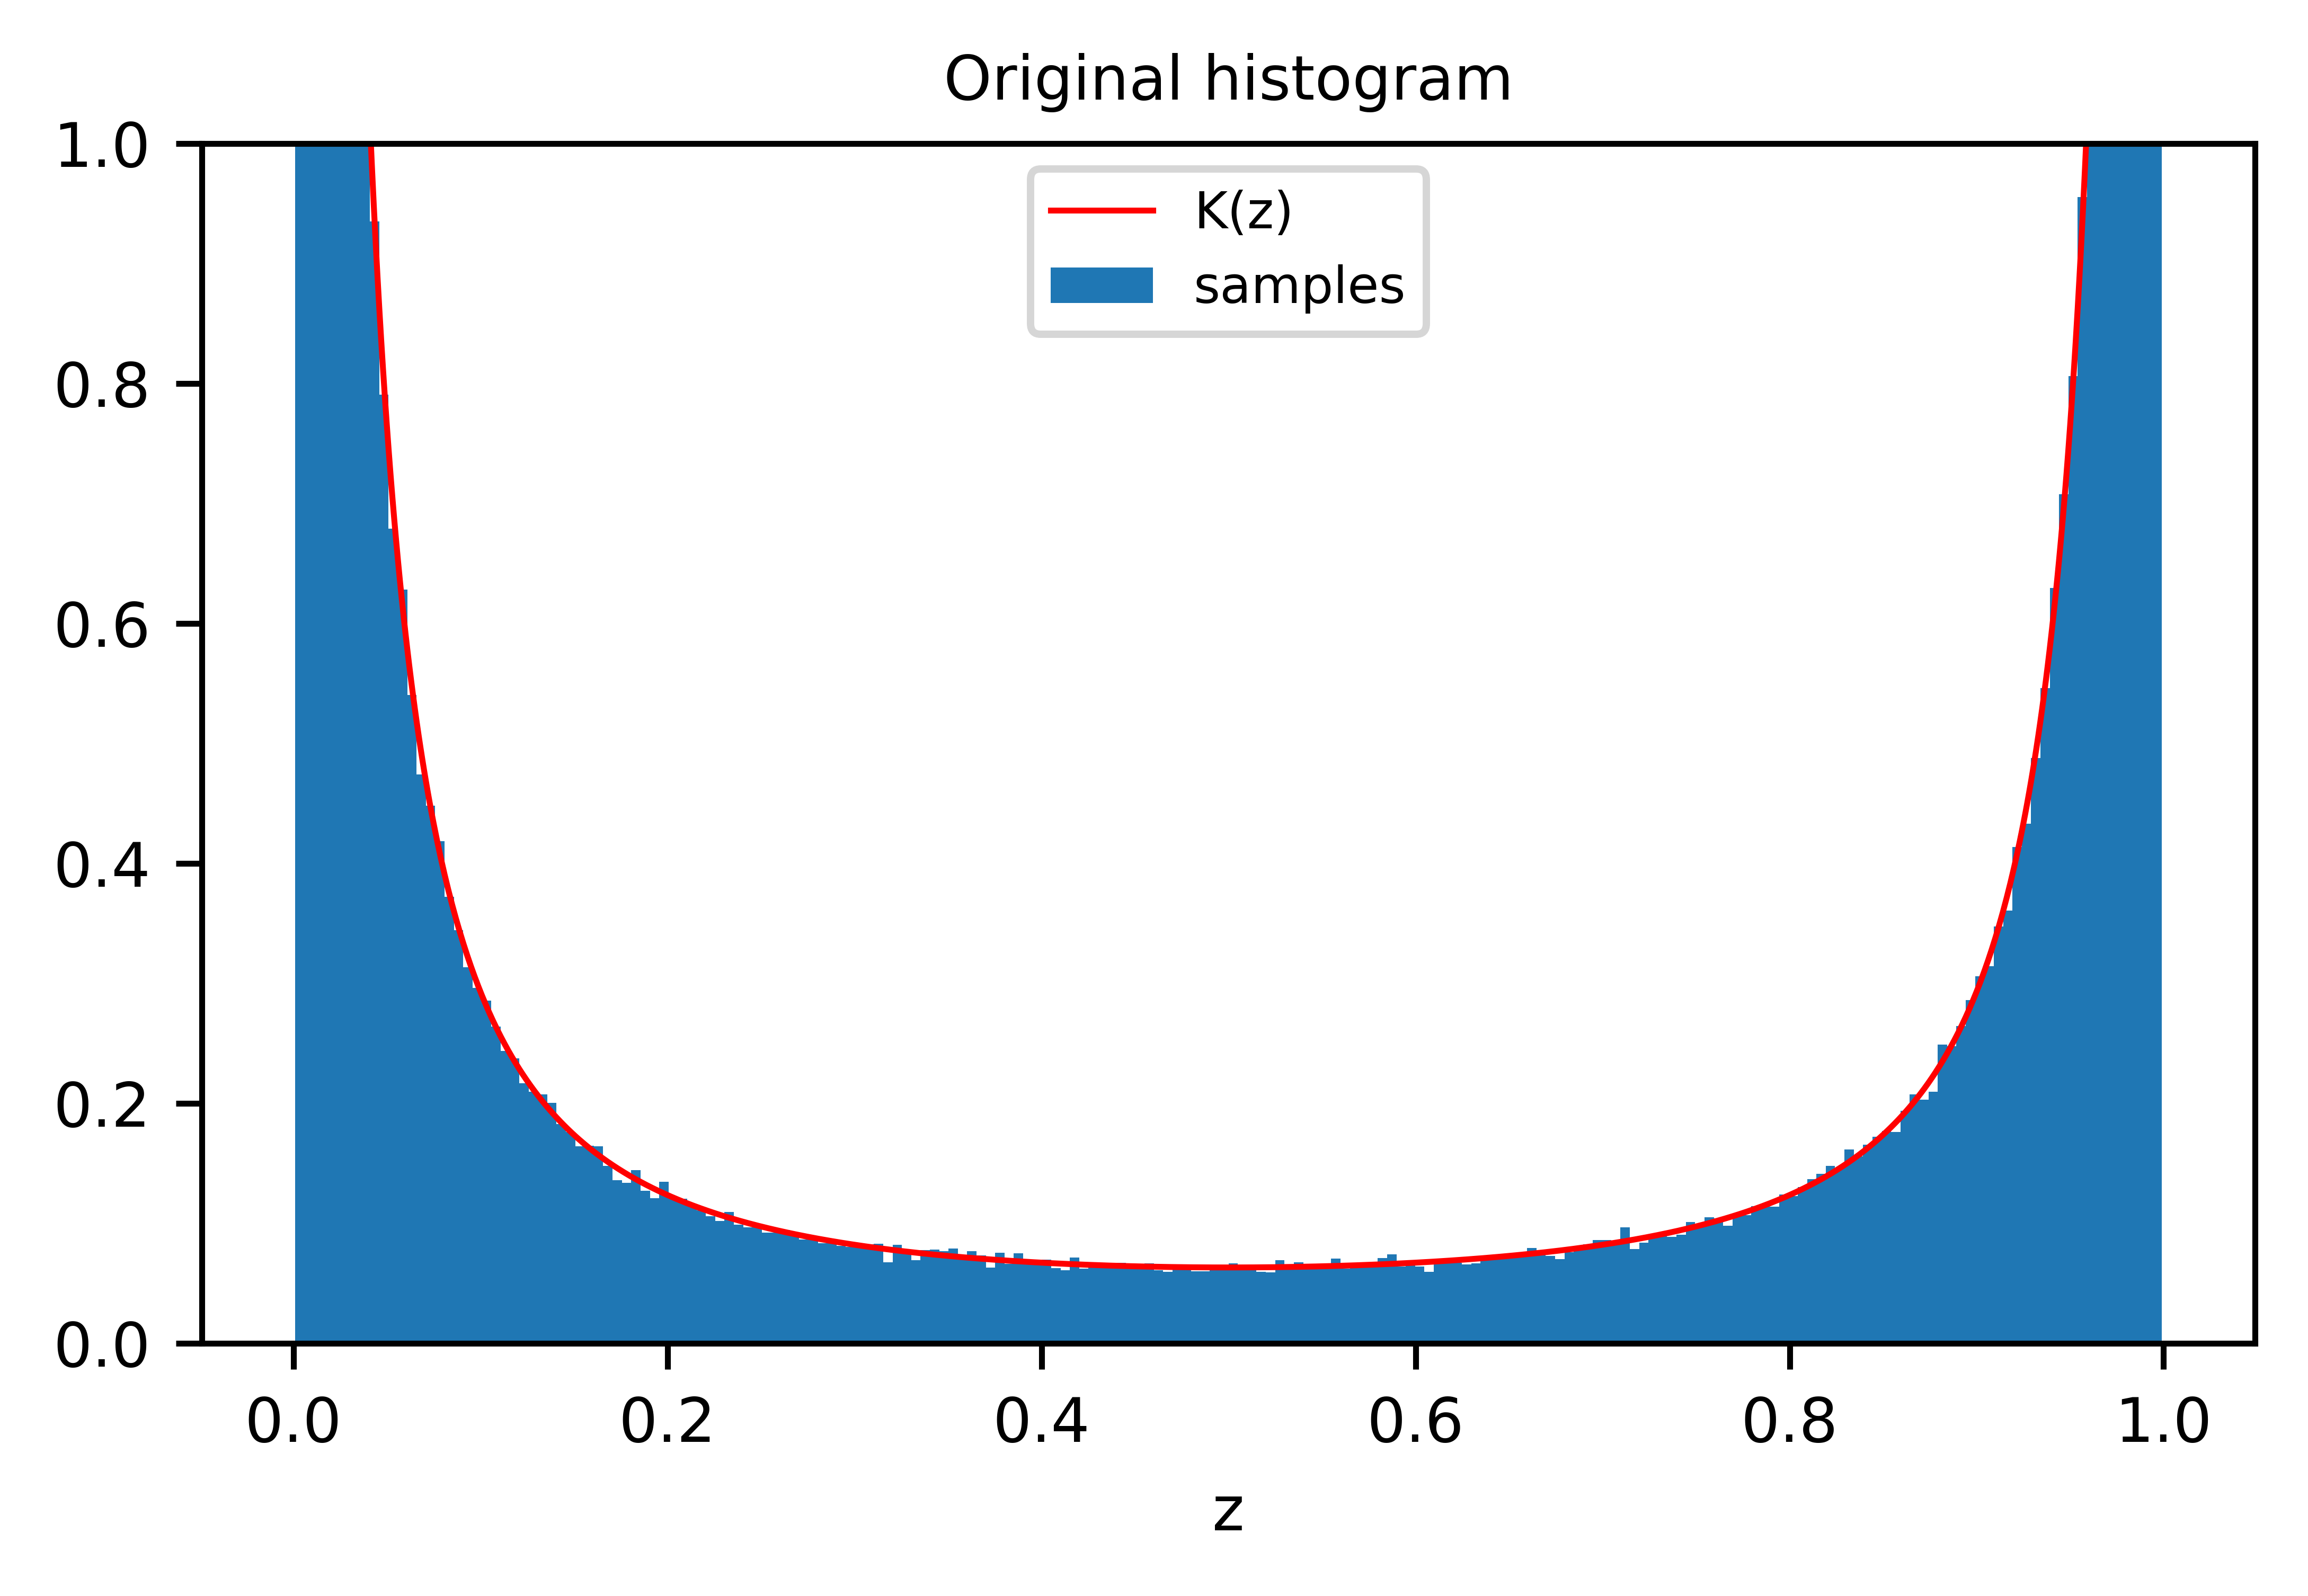
\includegraphics[width=9cm]{pictures/plots/splitting_functions/medium_gg_samples.png}
    \caption{Probability density of the simplified \(\mathcal{K}_{gg}(z)\) splitting kernel, and the histogram of sampled values using \autoref{eqn: medium_gg_sampling}. Simulated with \(10^6\) samples.}
    \label{fig: medium_gg_sampling}
\end{figure}

\subsection{Monte-Carlo implementation}
Creating the Monte-Carlo program for the medium showers follows generally the same procedure as in \autoref{sec: MC_implementation_vacuum}. As already discussed, we will restrict ourselves to gluons and the reduced kernel. There are some obvious differences, as we now need to generate evolution intervals from the in-medium rate Sudakov form factor from \autoref{eqn: BDMPS_probable_branching_interval_tau}, and need to sample from the reduced kernel \autoref{eqn: medium_gg_sampling}. 

The other parameters are very similar, but we will need a lower limit for how soft gluon can split. This is particularly important for the medium cascade, as very soft gluons will barely evolve \(\tau\) at all, due to the \(x\) dependence in the generated evolution interval, meaning the program would be incredibly slow without a \(x\)-limit.. This limit is simply introduced by not appending gluons with a momentum fraction less than \(z=10^{-3}\) to the list of splitting gluons. When the plots are made it is then important to keep in mind that we don't have precise data below this limit. 

The final program is again available in the author's GitHub repository~\cite{GitHub_thesis}.

\subsection{Results for gluon showers in medium}
This section will be dedicated to verifying the results from our medium showers. Very similar to the vacuum programs we will compare the generated distributions with the analytical solution of the evolution equations, and other properties present will be highlighted using different plots.

We will now plot the inclusive energy distribution \(D(x,\tau)\) from the Monte-Carlo parton shower, along with the analytical solution for the in-medium kinetic rate equation as obtained in \autoref{eqn: BDMPS_solution}. It is important to keep in mind that this solution is only valid for the reduced kernel. The resulting plot is given with a linear scale in \autoref{fig: medium_gluoncomparison_analytical_lin}. The Monte-Carlo results are in generally good agreement with the analytical solution. 
\begin{figure}[htb]
    \centering
    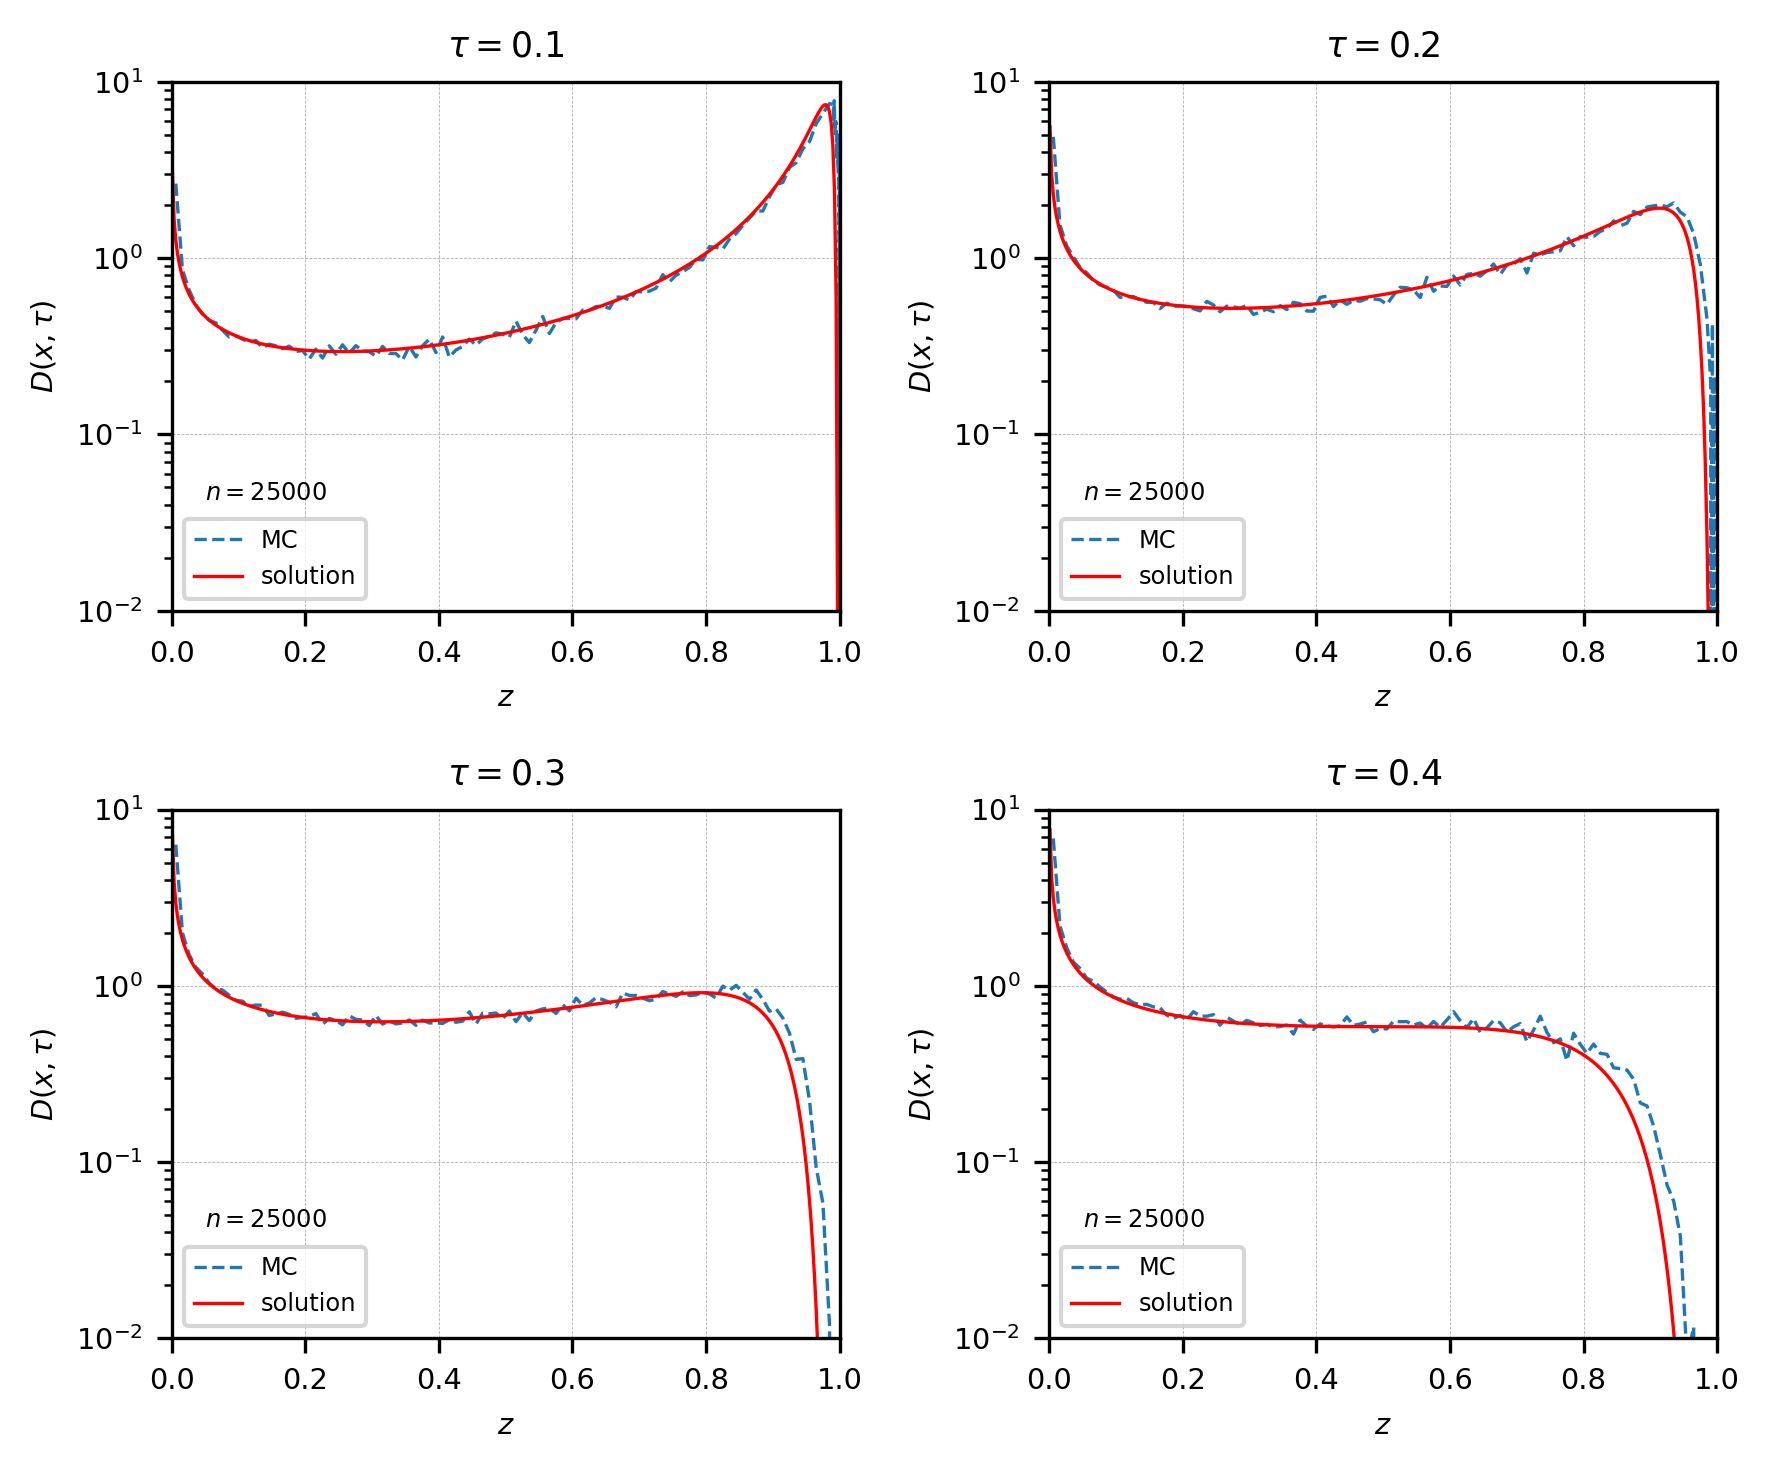
\includegraphics[width=13cm]{pictures/plots/distributions/medium/medium_shower__25k_lin.png}
    \caption{The inclusive energy distribution \(D(x,\tau)\) as generated from the Monte-Carlo program for gluons in medium, using the reduced kernel. Simulated with \(n=2.5 \cdot 10^4\) showers, using \(\epsilon=10^{-3}\) and \(z_{\text{min}} = 10^{-3}\). The distribution is compared with the analytical solution given in \autoref{eqn: BDMPS_solution}.}
    \label{fig: medium_gluoncomparison_analytical_lin}
\end{figure}

For observing the scaling property of the medium evolution, we will plot the distribution for different values of \(\tau\), on a logarithmic scale. This is presented in \autoref{fig: medium_comparison_scaling}. The scaling properties of the medium evolution is apparent for large values of \(\tau\), as once the peak corresponding to the initial parton around \(z=1\) has disappeared, the flow of energy towards small \(x\) values seems to be constant. As we discussed in \autoref{sec: BDMPS_properties}, the distribution changes in a uniform and shape-conserving way, once \(\tau\) goes larger than \(\tau \sim 1\). 
\begin{figure}[htb]
    \centering
    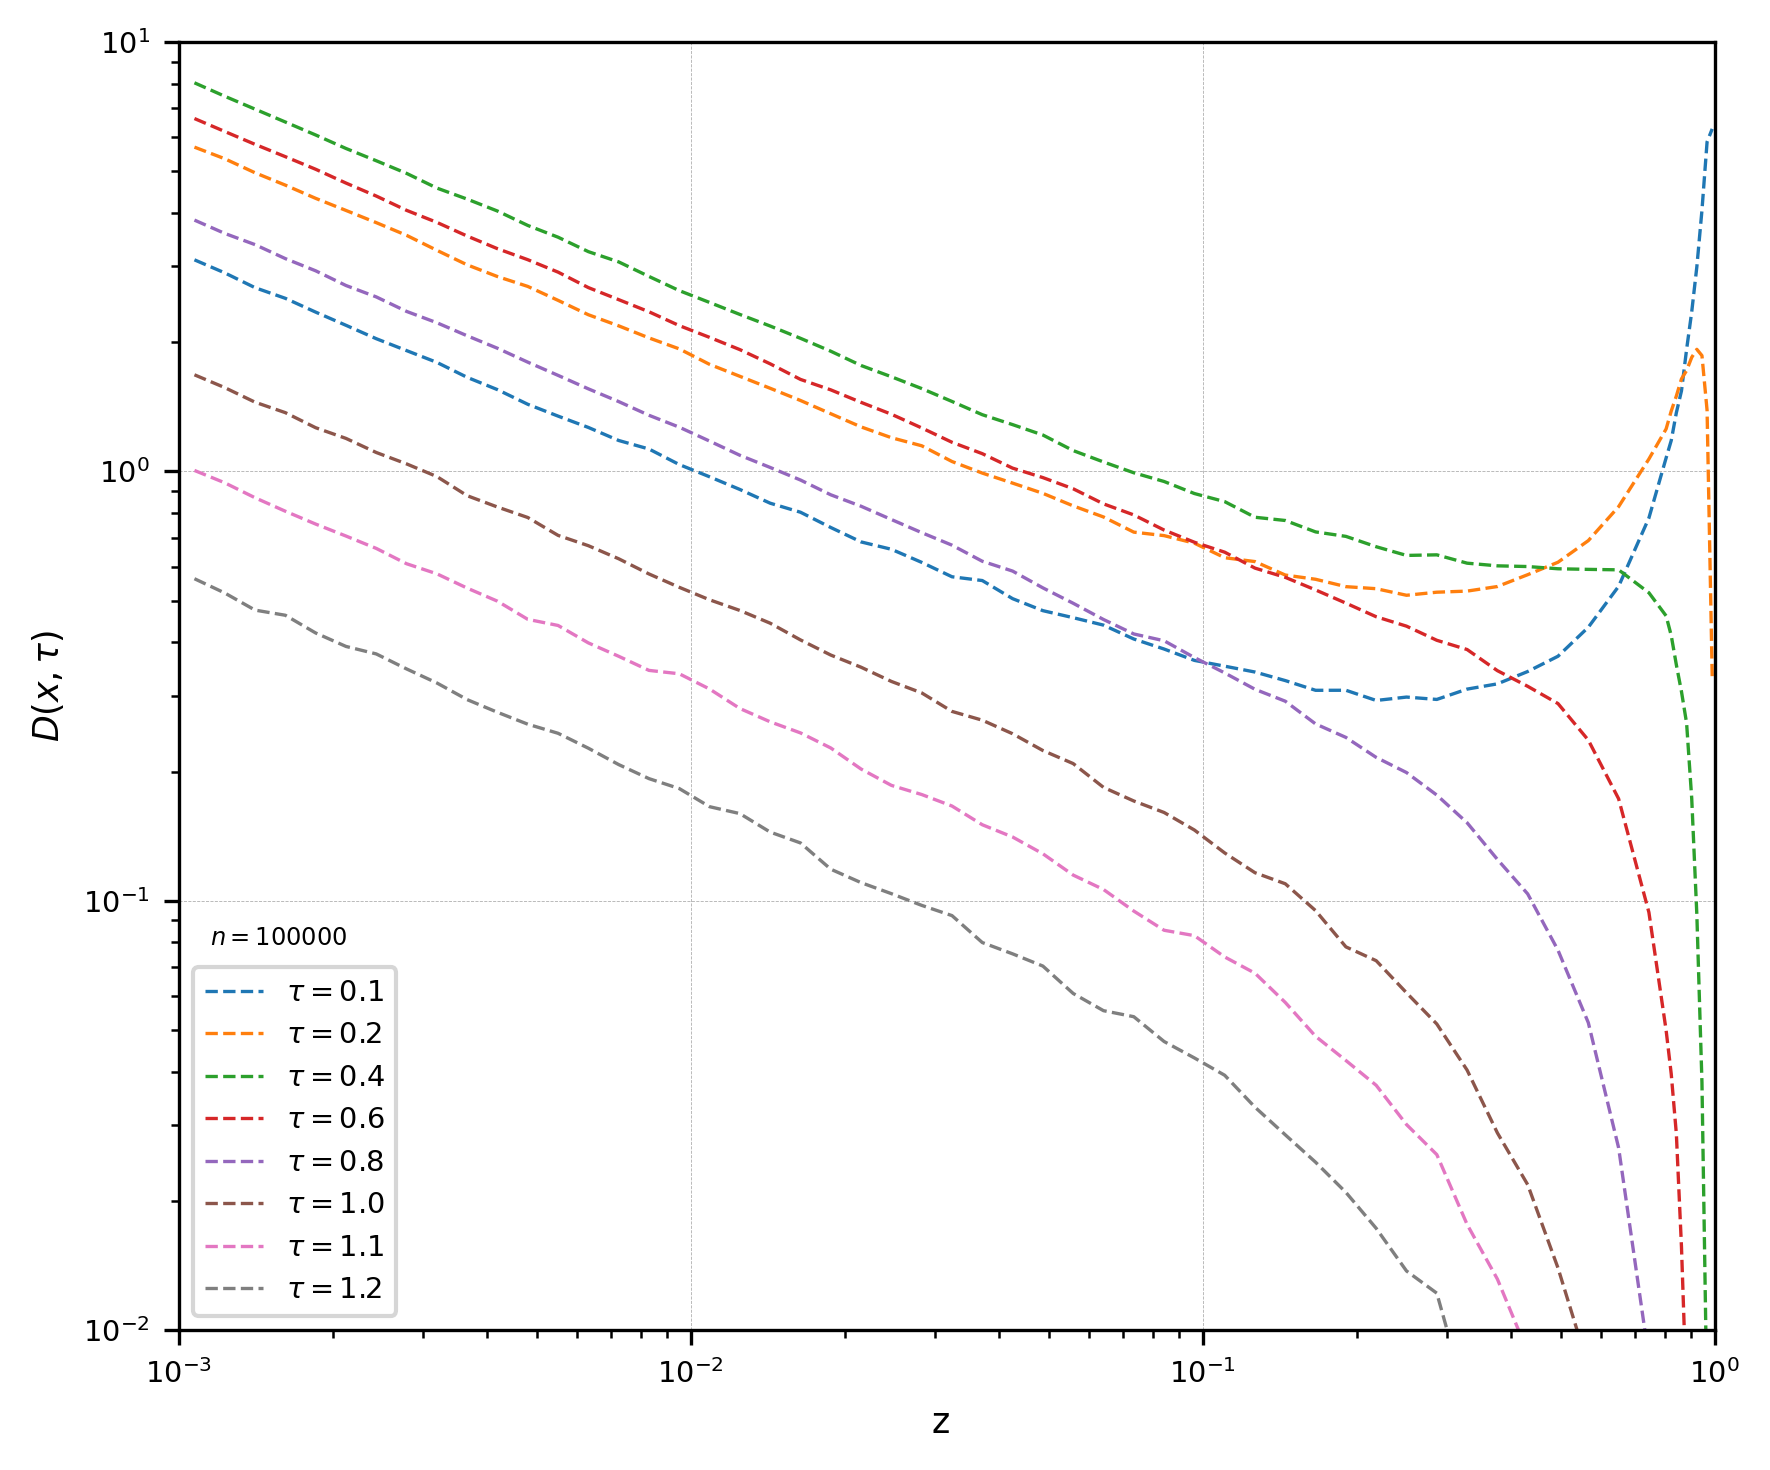
\includegraphics[width=10cm]{pictures/plots/distributions/medium/medium_scaling_100k.png}
    \caption{The inclusive energy distribution \(D(x,\tau)\) as generated from the Monte-Carlo program for gluons in medium, using the reduced kernel. Simulated with \(n=10^5\) showers, using \(\epsilon=10^{-3}\) and \(z_{\text{min}} = 10^{-3}\), for a wide range of values \(\tau\). The scaling property of the shower is apparent for values of \(\tau > 1\).}
    \label{fig: medium_comparison_scaling}
\end{figure}


\end{document}